\graphicspath{ {./Chapter 3/figures/erosion/}{./Chapter 3/figures/terrain_representations/}{./Chapter 3/results/}{./Chapter 3/otherPapersRepro/} {./Chapter 3/images/erosion_processes/}}

\newcommand{\referenceExemple}[1] {\textit{\cref{tab:erosion_result_figures}: #1}}
\newcommand{\addingFiguresToCell}[4]{%
        \includegraphics[width=0.2\textwidth]{#1}
        \includegraphics[width=0.2\textwidth]{#2}
        \ifx\relax#3\relax
        \else
            \includegraphics[width=0.2\textwidth]{#3}
        \fi
        \ifx\relax#4\relax
        \else
            \includegraphics[width=0.2\textwidth]{#4}
        \fi
}

% The columns :
% Name & Results & Terrain representation & Dimensions & particles / iteration & iterations & particle radius & coefficient of restitution & particle density & capacity factor & erosion factor & deposition factor & Velocity field & computation time
\newcommand{\exampleCoastal}{
Coastal & \addingFiguresToCell{Coastal_1.png}{Coastal_2.png}{Coastal_3.png}{} & \densityVox & 100x100x30 & 10 & 80 & 3 & 5 & 0.1 & 500 & 10.0 & 5.0 & 0.5 & Uniform & 0.5
}
\newcommand{\exampleGlacier}{
Glacier & \addingFiguresToCell{Glacier1.png}{Glacier2.png}{Glacier3.png}{Glacier4.png} & \heightmap & 100x100 & 20 & 80 & 3 & 10 & 0.1 & 500 & 1.0 & 1.0 & 1.0 & None & 0.8
}
\newcommand{\exampleLandslide}{
Landslide & \addingFiguresToCell{Glacier_2_1.png}{Glacier_2_2.png}{Glacier_2_3.png}{Glacier_2_4.png} & \heightmap & 100x100 & 20 & 200 & 10 & 2.5 & 0.2 & 500 & 0.1 & 1.0 & 1.0 & None & 4
}
\newcommand{\exampleHydraulic}{
Rain & \addingFiguresToCell{Hydraulic1.png}{Hydraulic3.png}{Hydraulic5.png}{Hydraulic7.png} & \heightmap & 100x100 & 20 & 100 & 10 & 1.0 & 1.0 & 1000 & 10.0 & 2.5 & 0.3 & None & 4.0
}
\newcommand{\exampleKarstBinary}{
Karst & \addingFiguresToCell{KarstBinaryWithMarchingCubes1.png}{KarstBinaryWithMarchingCubes2.png}{KarstBinaryWithMarchingCubes3.png}{KarstBinaryWithMarchingCubes5.png} & \binaryVox & 100x100x50 & 2 & 1000 & 40 & 5 & 0.5 & 500 & 10.0 & 5.0 & 0.5 & Uniform & 20
}
\newcommand{\exampleKarstBinaryStrata}{
Karst & \addingFiguresToCell{KarstWithStrataNoise1.png}{KarstWithStrataNoise2.png}{KarstWithStrataNoise3.png}{KarstWithStrataNoise4.png} & \binaryVox & 100x100x50 & 2 & 80 & 3 & 10 & 0.1 & 500 & 10.0 & 5.0 & 1.0 & Uniform & 0.8
}
\newcommand{\exampleLabyrinthOF}{
Glacier & \addingFiguresToCell{LabyrinthOpenFOAM1.png}{LabyrinthOpenFOAM2.png}{LabyrinthOpenFOAM3.png}{LabyrinthOpenFOAM4.png} & \densityVox & 100x100x40 & 2 & 80 & 3 & 10 & 0.1 & 500 & 1.0 & 1.0 & 1.0 & SIMPLE\cite{Caretto1973} & 0.8
}
\newcommand{\examplePipes}{
Tunnel & \addingFiguresToCell{Pipes01.png}{Pipes05.png}{Pipes09.png}{Pipes11.png} & \densityVox & 100x100x50 & 1 & 100 & 100 & 2.5 & 0.1 & 500 & 1.0 & 1.0 & 1.0 & None & 0.8
}
\newcommand{\exampleRiver}{
River & \addingFiguresToCell{River1.png}{River2.png}{River3.png}{River4.png} & \heightmap & 100x100 & 5 & 100 & 50 & 1.5-5 & 0.5 & 900 & 0.1 & 1.0 & 1.0 & None & 2.5
}
\newcommand{\exampleRiverTwo}{
River & \addingFiguresToCell{River_2_1.png}{River_2_2.png}{River_2_3.png}{River_2_4.png} & \heightmap & 100x100 & 5 & 100 & 50 & 1.5-5 & 0.5 & 900 & 0.1 & 1.0 & 1.0 & None & 2.5
}
\newcommand{\exampleRiverWater}{
\makecell{River\\(with water\\level)} & \addingFiguresToCell{RiverWater1.png}{RiverWater2.png}{RiverWater3.png}{RiverWater4.png} & \heightmap & 100x100 & 5 & 100 & 50 & 1.5-5 & 0.5 & 900 & 0.1 & 1.0 & 1.0 & None & 2.5
}
\newcommand{\exampleRiverObstacle}{
\makecell{River \\with obstacle} & \addingFiguresToCell{RiverWithObstacle1.png}{RiverWithObstacle2.png}{RiverWithObstacle4.png}{RiverWithObstacle6.png} & \heightmap & 100x100 & 5 & 100 & 50 & 1.5-5 & 0.5 & 900 & 0.1 & 1.0 & 1.0 & None & 2.5
}
\newcommand{\exampleWaterCurrents}{
Underwater & \addingFiguresToCell{WaterCurrent1.png}{WaterCurrent2.png}{WaterCurrent4.png}{WaterCurrent6.png} & \heightmap & 100x100 & 10 & 100 & 50 & 2.5 & 0.9 & 1000 & 1.0 & 1.0 & 1.0 & \cite{Stam2003} & 4
}
\newcommand{\exampleWindErosion}{
Wind & \addingFiguresToCell{WindErosion1.png}{WindErosion2.png}{WindErosion4.png}{WindErosion5.png} & \densityVox & 100x100x50 & 0.2 & 100 & 10 & 1.5 & 0.9 & 1.5 & 1.0 & 1.0 & 1.0 & \cite{Paris2019} & 0.5
}
\newcommand{\exampleVolcano}{
Volcano & \addingFiguresToCell{Volcano_2_1.png}{Volcano_2_2.png}{Volcano_2_3.png}{Volcano_2_4.png} & \densityVox & 100x100x40 & 50 & 150 & 30 & 1.0 & 5.0 & 2000 & 1.0 & 1.0 & 5.0 & None & 0.8
}
\newcommand{\exampleMeanders}{
Meanders & \addingFiguresToCell{meanders_base.png}{meanders_fin.png}{}{} & \implicit & N/A & N/A & 10 & 20 & 5.0 & 1.0 & 1000 & 1.0 & 1.0 & 1.0 & $^{(1)}$ & 1
}


\chapter{Erosion simulation}
\label{chap:erosion}

\teaser {
	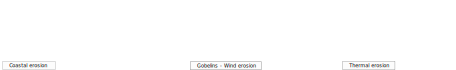
\includegraphics{teaser.pdf}
	\centering
	\caption{Applying shading and textures on the generated geometry can produce a plausible aspect of a coast eroded by waves on a long timespan, or a desertic landscape eroded by wind, or a mountainous area flatten by thermal erosion.}
	\label{fig:erosion_closerImage}
}

\abstract
% - Work carried out at the beginning of the thesis \\
% - Representation choice still uncertain \\
% - Search for abstraction of the representation \\
% ** Drives the generalization of the erosion system

In this chapter, we present a novel particle-based method for simulating erosion on various terrain representations, including height fields, voxel grids, material layers, and implicit terrains. Our approach breaks down erosion into two key processes - terrain alteration and material transport - allowing for flexibility in simulation. We utilize independent particles governed by basic particle physics principles, enabling efficient parallel computation. For increased precision, a vector field can adjust particle speed, adaptable for realistic fluid simulations or user-defined control. We address material alteration in 3D terrains with a set of equations applicable across diverse models, requiring only per-particle specifications for size, density, coefficient of restitution, and sediment capacity. Our modular algorithm is versatile for real-time and offline use, suitable for both 2.5D and 3D terrains.
\pagebreak

\minitoc

\section{Introduction}
Automated terrain generation is a key component of natural scene digital modeling for animated movies and video games. A standard approach is to first generate a base terrain geometry using noise to define the height on the input domain \cite{Musgrave1989, Olsen2004, Roudier1993}, the result will most likely lack realism and feel synthetic. Erosion simulation algorithms are applied, to simulate thousands of years of ageing by reproducing physical phenomena - i.e. effects of the elements (rain, wind, running water...) - affecting the terrain making it more believable \cite{Stachniak2005, Smelik2009, Galin2019}.\\
The process of terrain alteration caused by the effect of water, air, or any other element - natural or not - over time is usually performed in three steps \cite{Neidhold2005}: \textbf{detachment} - pieces of the ground of variable dimensions, ranging from complete ledges to grains of sand, are removed from the terrain depending on the simulated meteorological phenomenon - \textbf{transport} - pieces of ground fallen from their initial position are moved to a different one (e.g. a cornice falls down a slope or a grain of sand is thrown into the air) - and \textbf{deposition} - transported pieces of land are accumulated at a new part of the landscape. Various phenomena can cause these alterations: \textbf{thermal erosion} (bursting of rocks caused by expansion of water under frost, then falling of debris to the bottom of a slope), \textbf{hydraulic erosion} (detachment caused by the impact of water particles on surfaces and the transport of sediments by the flow of runoff), \textbf{wind erosion} (fine particles carried away in the wind and hit surfaces on their way, creating new fine particles which then also fly away), \textbf{chemical erosion} (chemical decomposition of rocks caused by rainwater or other fluids), other exceptional phenomena such as avalanches, animals, lightning, etc... modify the terrain \cite{Cordonnier2017a, Argudo2020, Cordonnier2018, Cordonnier2017b,Cordonnier2023}. 

\begin{figure*}
\centering
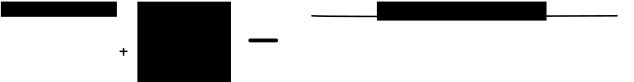
\includegraphics{pipeline.png}
\caption{Our method require a base geometry, a small number of parameters for the particles and the medium used for the erosion simulation. It can be easily adapted to be compatible with different mediums and terrain representations.}
\label{fig:erosion_pipeline}
\end{figure*}

In practice, the core idea to simulate erosion is to add or remove material from the terrain at given positions on the interface between the terrain and fluid eroding it (e.g. air or water). Hence, the two major problems to tackle are: how to locally alter the terrain geometry for material detachment and deposition and where to perform these alteration given the properties of the environment (terrain slope, fluid density and velocity).
A terrain is more than often represented in 2.5D using a 2D image called a heightmap which grey scale values define terrain elevation. While being the major terrain representation, only a limited number of environments can be modeled. Indeed, natural landscapes are intrinsically 3D (overhangs, cavities or geological structures such as arches or gobelins), this is particularly true for underwater environments generation. Alternate representation such as voxel grids, material layers or implicit surfaces can be used. A wide variety of method have been proposed to simulate natural erosion phenomena on heightmaps as the partial differential equations to model erosion can be discretized and solved in 2D and the material detachment and deposition at a given point of the terrain surface can be easily performed by elevating or lowering the ground level i.e. changing locally pixel intensities. 
For volumetric representations, the alteration of the terrain is not as trivial.
To define where to perform the erosion process the local slope variations are more than often used combined with eroding medium information. This fluid can be simulated using particle systems, Smoothed Particle Hydrodynamics (SPH) \cite{Kristof2009} or approximated using a simple vector field. 
Proposed methods offer a specific erosion effect tailored to a single terrain representation and fluid simulation.

In this work we propose an approach to simulate a large part of the geomorphological and meteorological phenomena present in the literature of terrain generation (including 3D and volumetric effects). We introduce a generalized algorithm performing the three stages of erosion on surface and volume representations alike, and expose very few intuitive parameters to be adjusted by the user (\cref{fig:erosion_pipeline}).
We propose to tackle separately the material variation and the fluid simulation. Our method relies on a particle system to simulate eroding agents, each thrown particle will collide with the terrain, perform terrain alteration at the collision point and transport material along its path. 
Their motion is computed using simple particle physics accounting for the medium density and particle properties (buoyancy and gravity forces). We consider each particle as independent, hence, they do not interact with each other, no collision detection or response. This simplification allows for efficient parallel computation. 
When more accuracy or control is needed, we propose to provide a vector field used to modify the particle speed at each time step. The nature of this vector field is flexible, it can be computed using a more or less accurate fluid simulation (SPH, FLIP,...) or be manually defined by the user. We propose a particle-based strategy for material alteration that can be applied on surface and volumetric representation. \\
The main contributions of this chapter are: 
\begin{itemize}
\item a generalized particle-based algorithm performing the three
stages of erosion on surface and volume representations,
\item decoupling the erosion system from the fluid simulation, making the process more flexible in its usage and implementation and opening the door for richer effects that can easily be produced.
\end{itemize}
% -----------------------------------------------------------------

\section{Erosion}
Erosion is the complex, gradual process through which natural forces such as water, wind, ice, and gravity wear away soil, rock, and sediment, transporting these materials across the landscape and leading to significant changes in topography and landform structure over time. This process, fundamental to both natural and human-modified environments, involves several interacting factors, including the type and composition of surface material, climate conditions (such as precipitation, temperature fluctuations, and wind intensity), topography (including slope steepness and aspect), and the presence of vegetation.

Studying erosion is essential across numerous fields due to its impact on landscapes, ecosystems, infrastructure, and resource sustainability. In agriculture, for example, erosion poses a direct threat to soil fertility and crop productivity, driving the need for conservation practices that retain topsoil and prevent land degradation. In civil and environmental engineering, erosion control measures are fundamental to maintaining the stability of roads, bridges, and coastal structures, safeguarding both urban and rural infrastructure. Similarly, urban planning incorporates erosion management into green infrastructure and stormwater systems to protect densely populated areas from soil loss and water damage. Ecologically, erosion shapes habitat stability and biodiversity, affecting riverine, forest, and coastal ecosystems; as a result, restoration efforts are vital to sustain healthy landscapes and support species diversity. In water resource management, erosion control is integral to preventing sedimentation, preserving water quality, and managing flood risks, which are essential for both environmental health and human safety. Within climate science, erosion is studied for its role in the carbon cycle, land degradation, and desertification, as it influences carbon release and soil loss in vulnerable areas. Erosion is also a key focus in natural disaster risk assessment, where slope stability and riverbank management are crucial for preventing landslides and floods that could endanger communities. Furthermore, in mining and resource extraction, erosion control mitigates environmental damage by supporting ecosystem recovery and reducing sediment pollution in surrounding areas. [ADD CITATIONS FOR EACH FIELD].

The effects of erosion extend beyond simple landscape alteration. They play a central role in soil formation, nutrient cycling, and the distribution of sediments in various ecosystems.

The main problem with studying erosion is the large amount of factors to take into account in the process. When studying erosion, a range of interconnected properties must be considered to understand its causes, rates, and impacts. Soil and rock characteristics such as texture, structure, cohesion, permeability, and organic matter content influence how easily soil and sediment detach and are transported. Climate factors like rainfall intensity, temperature fluctuations, wind speed, and seasonal changes impact erosion by affecting soil moisture and stability. Topography—including slope gradient, length, elevation, and drainage patterns—affects how water flows and gathers momentum, directly influencing erosion potential. Hydrological factors like surface runoff, infiltration rate, groundwater flow, and wave action are critical in understanding how water drives erosion in riverine and coastal environments.

Biological influences include vegetation cover, root density, and plant types, which stabilize soil, while animal activities like burrowing can increase erosion susceptibility. Human activity, such as agriculture, deforestation, urbanization, and mining, significantly accelerates erosion by disturbing soil and removing natural vegetation. Geological properties like soil depth, rock layering, and prior erosion events, along with chemical characteristics such as mineral composition and soil acidity, also shape erosion patterns, influencing how landscapes respond to environmental forces. Temporal factors—including the duration of exposure, rate of soil formation, seasonal cycles, and the frequency of intense weather events—affect erosion rates over time, leading to varying erosion impacts across regions and ecosystems. These properties collectively provide a comprehensive foundation for understanding and managing erosion processes across diverse landscapes.

Due to the large amount of properties to take into account, each domain uses a subset of the factors, with more or less simplifications in the erosion model. Depending on the use case, the analysis of erosion effects may vary largely. [ADD EXAMPLE OF FIELDS THAT STUDY EROSION THAT HAVE INSTANTANEOUS EFFECTS LIKE LANDSLIDES AND FIELDS THAT USE MILLIONS OF YEARS LIKE TECTONIC ACTIVITY].

In procedural terrain generation, simulating erosion based on soil and rock characteristics (like texture, cohesion, and permeability) allows the algorithm to mimic how different materials break down and redistribute under various conditions. For example, regions with sandy or loosely cohesive soils can be programmed to erode more rapidly, while rocky, cohesive areas remain more stable.

Incorporating climate factors (rainfall, wind, and temperature) helps to model how landscapes evolve in different biomes—such as dry, windy deserts versus lush, wet valleys. Simulating topographic influences like slope gradient and drainage patterns enables the formation of natural-looking valleys, cliffs, and river networks, while accounting for hydrological factors like runoff and groundwater flow creates realistic water paths and sediment deposits.

Procedural algorithms can also use biological factors to define erosion resistance based on vegetation cover, with densely vegetated areas exhibiting slower erosion rates and barren regions eroding faster. Including human activity effects, such as altered runoff or deforestation, allows for terrain that mirrors landscapes influenced by development or agriculture, adding further realism. Finally, using temporal properties to simulate seasonal erosion and landscape changes enables the terrain to evolve naturally over time, creating dynamic environments where erosion patterns shift as weather and vegetation change.





\section{State of the art}
\label{sec:erosion_state_of_the_art}
In this section, we first present the major terrain representations (height fields, layered representations, voxel grids, and scalar functions) and a subset of the major simulated phenomena used to erode terrains. We highlight the fact that, in the literature, a specific erosion method tailored to a given terrain representation is proposed for given phenomena which might lead to limitation in term of terrain modeling. Indeed, changing representation costs information and precision loss.

\subsection{Terrain representations}

Terrain refers to the physical features and configuration of a specific area of land. It includes the elevation, slope, and the overall topography, such as mountains, valleys, and plains. Terrain is often used to describe the surface characteristics of the land, focusing on the natural contours and the geographical aspects that define a region's physical form.

While the term "terrain" describes the physical characteristics of land, it does not include the natural elements that shape an area's identity. Elements like vegetation, water bodies, and climatic conditions, such as snow cover, are essential to how we perceive and understand a landscape. Therefore, when discussing procedural generation in virtual environments, "landscape generation" is a more fitting term, as it integrates these natural elements along with the topographical features.

In addition to "terrain generation," other terms such as "landscape generation," "world generation," and "environment generation" can be used to describe the creation of virtual landscapes. These terms are interchangeable and can all refer to the process of generating physical terrain along with natural and artificial elements. However, by convention and for simplicity, the term "terrain generation" is most commonly used in the field. Despite its original focus on the physical features of the land, "terrain generation" has evolved to encompass a broader range of environmental elements, making it a convenient and widely accepted term for describing the comprehensive process of creating virtual environments.

A terrain can be represented in various ways, each of them suited for a given application of which we give an brief overview, more details can be found in \cite{Galin2019}.

\subsubsection{Elevation models}

\begin{figure}[h]
    \centering
    \includegraphics[width = 0.8 \linewidth]{elevation_representation.png}
    \caption{Elevation functions}
    \label{fig:erosion_elevation-representation}
\end{figure}

Elevation models are a fundamental approach in terrain representation, widely used in procedural generation due to their simplicity and efficiency. These models define the terrain as a function $h : \R^2 \to \R$, where each point in a 2D plane is mapped to an elevation value. This approach is particularly effective for representing terrains where the elevation is the only varying factor, such as hills, valleys, and plateaus, and it is best suited for terrains without complex 3D features like overhangs or caves. While we visualize elevation models in three dimensions, they are mathematically considered two-dimensional functions. In the domain of terrain generation, we will name them 2.5D models.

Elevation models are widely used in industries where large-scale terrain representation is crucial. In video games, they provide the foundation for creating vast open-world environments. In geographic information systems (GIS) and remote sensing, height fields are used to represent real-world terrain data, offering a practical means of visualizing and analyzing geographical features. The ability to manipulate and control terrain features procedurally makes elevation models a common choice for applications that require efficient terrain generation and rendering.

They offer a powerful method for representing terrains in procedural generation, combining simplicity with flexibility. While they have limitations in representing complex 3D structures, their efficiency and compatibility with existing algorithms make them indispensable in a variety of applications.

\subsubsubsection{Implicit height fields}

\begin{wrapfigure}{L}{0.4\textwidth}
    \includegraphics[width=\linewidth]{primitives_representation.png}
    \caption{Primitives composition}
    \label{fig:erosion_primitives-representation}
\end{wrapfigure}

Implicit height fields represent the terrain as a mathematical function that provides a height value at any given point in the domain. These functions can be procedural or closed-form expressions, allowing for compact storage and infinite precision in theory. The elevation function allows for easy manipulation of terrain features, making it ideal for generating terrains that require smooth, continuous surfaces. However, the primary disadvantage is the computational complexity involved in evaluating the function, especially for large or highly detailed terrains. The challenge lies in constructing functions that can realistically represent large-scale terrains with complex landforms.

\subsubsubsection{Discrete height fields}
Discrete height fields, or explicit height fields, are one of the most prevalent methods for terrain representation. These models consist of a 2D grid where each cell contains a height value, representing the elevation at that point. Height fields are particularly advantageous because they are simple to implement and are directly compatible with many rendering techniques and hardware, but also due to their closeness with image processing, a domain studied for many decades now.

The main advantage of height fields is their ability to handle large datasets efficiently, providing a balance between memory usage and detail. However, they are limited by their inability to represent terrains with overhangs or caves, as each point on the grid can only hold a single elevation value. Additionally, height fields often require interpolation methods, such as bi-linear or bi-cubic interpolation, to reconstruct a continuous surface from the discrete grid points. 

\subsubsection{Volumetric models}

\begin{figure}[h]
    \centering
    \includegraphics[width = 0.8 \linewidth]{volumetric_representation.png}
    \caption{Volumetric functions}
    \label{fig:erosion_volume-representation}
\end{figure}

Volumetric models represent a more complex approach to terrain modeling, allowing for the depiction of 3D features that go beyond the simple surface-based representation provided by elevation models. These models capture not only the surface of the terrain but also its internal structure, making them ideal for representing terrains with overhangs, caves, and other subsurface features. 

Volumetric models, including layered materials, voxel grids, and implicit models, are essential in applications where terrain complexity and detail are primordial. In geological simulations, these models allow for accurate representation of subsurface structures and processes. Voxel models are widely used in games that require dynamic terrain deformation, providing a rich interactive environment for players. Implicit models are favored in situations where smooth, continuous surfaces are needed [FIND OTHER USE CASES].

\subsubsubsection{Implicit volumetric models}
Implicit volumetric models describe the terrain's shape and features using an implicit function. The terrain is represented by a mathematical function $f: \R^3 \to \R$ that determines the terrain surface by evaluating to an isovalue, often zero. This function provides a continuous representation of the terrain, with points inside the terrain returning positive values and while points in the air evaluate to negative values. It allows for the seamless representation of complex terrain features, including caves, overhangs, and varying geological structures, which are impossible to represent with  elevation models.

One of the key advantages of implicit models is their ability to produce smooth surfaces without the need for discrete polygonal meshes, which can result in realistic and natural-looking terrains. However, the computational complexity of evaluating the implicit function, especially for large terrains, can be a significant drawback. Additionally, converting an implicit surface into a mesh for rendering can be challenging and resource-intensive. \cite{Araujo2015} 

\subsubsubsection{Layered models}
Layered models are a type of volumetric representation that encode different material layers within the terrain and are defined by a function $\mu : \R^3 \to \material$, where $\material$ denotes the material type at any given point in 3D space. This allows for a detailed representation of the terrain's internal composition, which can be crucial for applications requiring realistic geological simulations. Each layer is defined by its thickness or elevation, and multiple layers can be stacked to represent complex geological formations. These layers might include materials like bedrock, sand, soil, or water, each contributing to the overall structure of the terrain. Layered models are particularly useful in simulations that involve processes like erosion or sedimentation, where the interaction between different material layers affects the physical process.

The primary advantage of layered models is their ability to represent a stratified terrain with distinct material properties, which can be manipulated individually. This makes them well-suited for simulations that require detailed geological accuracy. However, they are more complex to implement than simple elevation models and require additional computational resources to manage the interactions between layers. 


\subsubsubsection{Voxel grid models}
Voxel grids are a common method for representing 3D terrains in procedural generation, offering the ability to capture complex internal structures and features that are difficult or impossible to represent with surface-based models. In a voxel grid, the 3D space is divided into a regular grid of small, cube-shaped elements called voxels (volumetric pixels). Each voxel holds information about the material or properties of the terrain at that specific point in space. This approach allows for detailed modeling of features such as caves, tunnels, overhangs, and intricate underground networks. The regular grid structure allows for the use of image processing-oriented algorithms.

There are three primary types of voxel grids used in terrain representation: binary voxel grids, material voxel grids and density voxel grids. Each has distinct characteristics, advantages, and limitations, making them suitable for different applications. 

\subsubsubsubsection{Binary voxel grids}
Binary voxel grids are the simplest form of voxel representation. In these grids, defined $f: \R^3 \to [0, 1]$, each voxel is either "filled" or "empty," representing the presence or absence of material. This binary state is typically represented by a 1 (filled) or 0 (empty). Binary voxel grids are straightforward to implement and require much less memory compared to more complex voxel representations, making them ideal for applications where the primary concern is whether a space is occupied or not.

The simplicity of binary voxel grids is one of their main advantages. They are easy to understand and visualize, with each voxel requiring only a single bit of information to represent its state. Additionally, because only a binary state is stored, these grids can be memory-efficient when combined with compression techniques like Sparse Voxel Octrees (SVOs) \cite{Laine2010} or voxel Directed Acyclic Graphs (DAG) \cite{Villanueva2017,Careil2020}. The simplicity of the data structure also allows for quick processing, making binary voxel grids suitable for real-time applications where performance is required. However, the binary nature of these grids limits their ability to represent variations in material density or properties, or even smoothness, resulting in less detailed terrain models. This can lead to hard, blocky edges in the terrain, which may appear unnatural without additional smoothing or processing.

\subsubsubsubsection{Material voxel grids}
Material voxel grids, defined as $\mu: \R^3 \to \material$, are commonly used in applications where simple occupancy information is sufficient. For example, voxel-based games like Minecraft utilize material grids to create terrains composed of solid blocks with clear boundaries. These grids are also employed in scientific simulations where the primary concern is the presence or absence of materials, rather than detailed material properties.

\subsubsubsubsection{Density voxel grids}
Finally, density voxel grids allow each voxel to store a range of values, representing varying degrees of material presence with $f: \R^3 \to \R$. Instead of a simple discrete state, a density voxel grid assigns a continuous value to each voxel, which can represent material density, opacity, or other properties. This added complexity enables density voxel grids to represent subtle variations in terrain, such as gradual changes in material density or smooth transitions between solid and empty spaces, allowing for more realistic and natural-looking terrain models.

% The use of density voxel grids results in soft transitions and smooth surfaces, reducing the blockiness typically associated with binary voxel grids. They are versatile and can represent not only solid terrain but also phenomena like fog, fluid densities, or temperature gradients. However, the increased detail and realism come at the cost of greater complexity. Density voxel grids require more memory and computational power, making them more challenging to implement and manage. The additional data and processing required can also lead to slower performance, particularly in real-time applications.

Density voxel grids are often used in high-fidelity simulations where detail and realism are essential. They are found in applications such as medical imaging, scientific visualizations, and advanced terrain modeling for films and visual effects. These grids are also employed in procedural terrain generation systems that require smooth and natural transitions between different terrain features, such as caves, cliffs, and eroded landscapes.







\subsection{Erosion processes}
Driven by an array of natural forces and processes, erosion varies significantly across environments, from the intense carving of river valleys to the subtle reshaping of slopes in arctic regions. In this section, we present the primary types of erosion—thermal, hydraulic, and wind erosion—alongside other significant processes that contribute to landscape change. Each erosion type not only influences distinct terrain forms but also varies in applicability depending on terrain representation in simulations. Notably, not all erosion types are easily adaptable to all forms of terrain representation, due to inherent limitations in data resolution and computational methods.

\subsubsection{Thermal erosion}
\wrapFig{freeze-thaw.jpg}{0.25}{fig:erosion-freeze_thaw}{Freeze-thaw process from \cite{Wang2017}}

Freeze-thaw weathering, also known as frost wedging or frost shattering, is a process that occurs when water infiltrates cracks and pores within rocks and then freezes. As the water freezes, it expands and exerts pressure on the rock, causing it to fracture and break apart over time. This cycle of freezing and thawing is especially prevalent in regions with large temperature variations between day and night or between seasons, such as alpine and polar climates. Over time, freeze-thaw weathering contributes to the breakdown of large rocks into smaller fragments, creating loose rock material that can accumulate and gradually move downslope.

Freeze-thaw weathering plays an important role in shaping landscapes, as it weakens rock faces and cliff edges, contributing to the formation of loose rock debris that eventually becomes part of other erosive processes, such as the development of talus slopes.

In procedural terrain generation, freeze-thaw weathering is approximated by simulating rock fragmentation along exposed edges. By iteratively introducing fractures and breaking down rock surfaces, models can create natural-looking debris fields and weathered cliff faces. This effect is achieved with algorithms that apply incremental degradation over time, though limitations in data resolution and computational resources often require simplifications in representing fine-scale debris patterns.

[More details about thermal erosion in PG]

This iterative approach enhances the visual realism of mountainous or polar landscapes, where freeze-thaw weathering significantly shapes terrain.


\subsubsection{Gravity-driven erosion}
\wrapFig{earthflow-erosions.jpg}{0.25}{fig:erosion-landslides_processes}{Different landslide processes}

Gravity-driven erosion encompasses processes that involve the downslope movement of soil, rock, or debris due to the force of gravity. These processes, including landslides and talus slope formation, play a crucial role in reshaping landscapes by redistributing materials across slopes, valleys, and cliffs, influencing terrain stability and morphology.

\subsubsubsection{Landslides}
Landslides encompass a range of processes where rock, soil, or debris moves downslope due to gravity. These events vary in scale and speed, ranging from rapid, sudden rockfalls to slow, gradual soil creep. They can be triggered by factors such as heavy rainfall, seismic activity, or thawing permafrost, which destabilize slopes and initiate movement. Key types of landslides include:
\begin{Itemize}
    
    \Item{Rockfalls:} Sudden detachment of rock from steep faces, often triggered by weathering, freeze-thaw cycles, or seismic activity, leading to rapid downslope movement. 
    \Item{Soil creep:} Slow, continuous downslope movement of soil and rock, caused by repeated cycles of expansion and contraction due to changes in moisture and temperature, often imperceptible over short timescales.
    \Item{Mudflows and debris flows:} Rapid flows of water-saturated soil and debris, typically triggered by heavy rainfall or snowmelt, which transport large volumes of material downslope in a short period.
\end{Itemize}
    
Landslides are a major force in landscape evolution, rapidly reshaping terrain and redistributing materials across slopes and valleys. They often follow periods of intense rainfall, seismic activity, or sudden thawing in permafrost areas, and are critical in maintaining slope stability over geological timescales.

In procedural terrain generation, landslides are simulated by identifying areas where slopes exceed stability thresholds, such as steep inclines or saturated soils. Simulations of rockfalls and debris flows involve detaching particles on steep slopes and allowing them to move downslope, responding to gravity. For gradual processes like soil creep, models apply small, iterative displacements to terrain layers, creating a subtle smoothing effect over time. These simulations, while effective in adding varied textures to terrains, often require simplifications due to the computational complexity of modeling real-time slope failures.

\subsubsubsection{Talus slopes}
\wrapFigR{talus.png}{}{}{} % {Mark A. Wilson (Department of Geology, The College of Wooster)}{fig:erosion-talus}

Talus slopes, also known as scree slopes, are accumulations of loose, angular rock debris at the base of cliffs, steep slopes, or mountainous areas. These slopes form as fragments of rock break off due to weathering processes like freeze-thaw and gravity pulls them downslope, where they accumulate in a cone-shaped deposit. Talus slopes are common in high-altitude or cold regions where physical weathering of rock faces is intense, and they contribute to the visual ruggedness of mountainous landscapes.

In procedural terrain generation, talus slopes can be simulated by redistributing rock fragments or particles to accumulate at the base of cliffs or steep inclines. This effect can be achieved by applying gravity-based algorithms that allow loose materials to fall and settle, forming natural slopes of debris at the base of rocky terrain. Talus slope simulation adds depth to mountainous landscapes, giving them a natural and weathered appearance.



\subsubsection{Hydraulic erosion}
\begin{figure}[h]
    \centering
    \includegraphics[width = 0.8 \linewidth]{hydraulic_erosion.pdf}
    \caption{Hydraulic erosion is tailored by the friction of water displacing sediments in a slope}
    \label{fig:erosion_hydraulic-erosion}
\end{figure}


Hydraulic erosion is the process by which moving water dislodges and transports soil, sediment, and rock from the Earth’s surface. Occurring in multiple forms, including river-based, rainfall-induced, and coastal erosion, hydraulic erosion is driven by factors such as water velocity, volume, and surface composition. This process plays a primary role in reshaping landforms—forming valleys, river channels, and coastlines—and significantly contributes to sediment redistribution in terrestrial and coastal environments.

2.5D terrains are widely studied for this simulation, using either water slope velocities \cite{Neidhold2005} or water simulations for erosion effects \cite{Mei2007}. For smaller scales, 3D fluid simulations on voxel grids have been proposed \cite{Benes2006}. Kristof et al \cite{Kristof2009} used SPH (Smoothed Particle Hydrodynamics) for meshless erosion simulations on various terrains. Their method involves numerous particle interactions, demanding significant computational power. Our approach draws inspiration from this but enhances efficiency by removing certain particle interactions.


\subsubsubsection{Fluvial erosion}
\wrapFigL{river_erosion.pdf}{0.25}{fig:erosion_river-erosion-profile}
{The erosion on the river bank is the combination of two processes: the detachment of the bottom of the sides, then the break of the upper coasts. }

Fluvial erosion is the process by which rivers and streams reshape the landscape by eroding, transporting, and depositing sediment. This phenomenon occurs as the kinetic energy of moving water exerts mechanical forces on the riverbed and banks, dislodging soil, rock, and sediment particles. The intensity of fluvial erosion is influenced by factors such as water velocity, discharge (the volume of water flowing per unit time), channel slope, and the composition of the riverbed and banks.

In steep, fast-flowing sections of a river, higher water velocities generate turbulent flow, which increases the river's capacity to dislodge and carry large particles. These particles, including gravel and pebbles, collide with the riverbed in a process called abrasion, grinding and wearing down the bedrock over time. Additionally, water exerts direct hydraulic pressure, especially in areas where currents are swift, prying apart rocks and sediment through hydraulic action. This is especially effective in widening channels and undercutting banks.

Fluvial erosion processes contribute to a dynamic reshaping of river channels, forming distinct landforms such as V-shaped valleys, canyons, and river meanders. Over time, rivers naturally balance their erosive energy with sediment transport and deposition, forming floodplains where sediment is deposited during seasonal overflows. In meandering rivers, erosion typically occurs on the outer curves of bends, where flow velocity is highest, while sediment deposition takes place on the inner curves, forming point bars. This continual interaction between erosion and deposition drives the lateral migration of meanders, altering the river's course across the landscape. The river’s competence, or its ability to transport particles of a certain size, depends on the flow’s velocity and discharge. During periods of high flow, such as after heavy rainfall or snowmelt, rivers gain greater erosive power, enabling them to transport larger particles and increase their erosion rates.


\subsubsubsection{Rainfalls}
\wrapFig{rillsGullies.jpg}{0.25}{fig:erosion-rills_gullies}{From \cite{Geertsema2010}}
Rainfall-induced hydraulic erosion begins as raindrops strike exposed soil surfaces, causing splash erosion, where particles are dislodged and displaced by the impact of individual raindrops, creating tiny craters \cite{Li2024}. As rainfall accumulates and flows overland, it transitions into sheet erosion, where a thin layer of water, known as sheet flow, moves across the land surface. This process is often intensified on sloped terrain, where the water gains momentum as it descends, picking up and carrying loose particles downslope. Sheet erosion can remove a uniform layer of soil across a large area, gradually depleting soil fertility and weakening the structure of the soil surface.

On steeper or more prolonged slopes, sheet flow may concentrate into small channels, initiating rill erosion. Rills are narrow, shallow channels that cut into the soil as water flow converges, carving miniature stream-like paths down the slope. As rills deepen and widen, they can evolve into larger channels in a process called gully erosion. Gullies represent a more severe stage of erosion, where channels become deep and wide enough that normal agricultural or natural processes cannot easily repair them. Gullies disrupt the landscape, fragmenting ecosystems, and accelerating the removal of topsoil.

The extent of erosion depends on factors such as rainfall intensity and duration, soil type, vegetation cover, and slope steepness. Sandy soils, for instance, are more prone to erosion due to their low cohesion, whereas clay-rich soils, while more resistant to initial splash erosion, are highly susceptible to rill and gully formation once water begins to concentrate.

\subsubsection{Chemical erosion and caves}

% \wrapFigR{corrosion_erosion.pdf}{0.25}{fig:erosion_corrosion-erosion}
% { ... }
\wrapFigR{seaCaveArch.jpg}{0.25}{fig:erosion_corrosion-erosion}{By Steve Hillebrand/U. S. Fish and Wildlife Service}

Chemical erosion, also known as chemical weathering, involves the chemical reactions between water and rock that lead to the dissolution and alteration of minerals within the rock. This process is especially significant in river and coastal environments, where water, often containing dissolved carbon dioxide, interacts with rocks like limestone and dolostone to form weak carbonic acid. This acid reacts with carbonate minerals, gradually breaking down the rock structure through a process called dissolution. Over time, this breakdown weakens rock formations, making them more susceptible to mechanical erosion by water.

Chemical erosion is particularly influential in the formation of karst landscapes, where the dissolution of carbonate rocks creates unique features such as caves, sinkholes, and underground drainage systems. As acidic water seeps into fractures within the rock, it slowly enlarges these cracks, leading to the creation of hollow spaces and intricate cave networks. In addition to carbonic acid, other dissolved ions, such as sulfur and organic acids, can also contribute to the chemical weathering of rocks in various environments.

One of the most common ways caves form is through chemical erosion, particularly in landscapes with carbonate rocks, such as limestone and dolostone. This process, often referred to as karstification, occurs when acidic groundwater interacts with carbonate minerals. As carbon dioxide from the atmosphere or soil dissolves into rainwater, it forms weak carbonic acid, which then seeps into rock fractures. Over time, the acidic water dissolves the rock, enlarging fractures and creating extensive underground networks.

This form of chemical erosion gives rise to karst caves, known for their complex formations, including stalactites and stalagmites formed by mineral deposits left behind by dripping water. Karst caves are some of the world’s most intricate and expansive cave systems, with notable examples including Mammoth Cave in the United States and the Škocjan Caves in Slovenia.


In coastal areas, chemical erosion works alongside mechanical processes to shape shoreline features. The saltwater in coastal environments can accelerate chemical weathering, especially in rocks rich in reactive minerals. This combined action of chemical and mechanical processes results in a dynamic coastal landscape that includes cliffs, sea arches, and tide pools. Over time, these chemical reactions weaken coastal rock formations, allowing wave action to further erode and shape the coastline.

Sea caves can form through the mechanical force of hydraulic action as waves continuously impact the shore. These sea caves develop along coastlines with cliffs, where wave energy focuses on weak points in the rock, such as fractures or softer rock layers. Over time, the pressure from waves and tides pries apart rock fragments, carving out hollow spaces within the cliffside.

This hydraulic action often works in conjunction with other processes, such as abrasion, where sediment carried by waves further grinds down the rock surfaces. Sea caves are commonly found in areas with high tidal energy, with examples like the Blue Grotto in Malta and the sea caves along California's coastline.

In desert environments, caves can also form through aeolian erosion, where wind-driven sand particles abrade rock surfaces. These aeolian caves are typically found in sandstone or other softer rocks, where strong, consistent winds gradually wear away the rock. Unlike chemical or hydraulic caves, aeolian caves are usually shallower and smaller, as the erosive force of wind is less powerful than water or acid-driven processes. However, these caves add unique features to desert landscapes, creating sheltered hollows that sometimes serve as habitats for desert wildlife.

An example of aeolian caves can be seen in the Navajo Sandstone formations of the southwestern United States, where wind erosion has carved intricate cave-like recesses and arches.


% Corrosion, or chemical erosion, in the context of hydraulic processes, refers to the chemical interactions between water and rock that lead to the dissolution or weakening of rock material. This form of erosion is common in river and coastal environments where water, often containing dissolved carbon dioxide, forms weak carbonic acid that reacts with minerals in rocks, particularly limestone. The chemical breakdown of rock through corrosion complements the mechanical forces of hydraulic erosion, making rocks more susceptible to further dislodgement and transport by water.

% Coastal erosion is the process by which wave action and tidal forces wear away and reshape coastlines, removing sediment and rock from beaches, cliffs, and shorelines. The energy from waves striking the shore can dislodge particles, leading to abrasion, where sediment carried by water further erodes rock surfaces. Over time, coastal erosion forms cliffs, caves, and other coastal landforms, and it is influenced by factors such as wave energy, sea level, coastal rock type, and shoreline configuration. Coastal erosion plays a vital role in shaping dynamic coastal landscapes, but it also poses challenges for coastal management due to its impact on infrastructure and habitats.

% Aeolian caves, though less common than those formed by water erosion, develop when wind-driven sand particles carve out hollows in softer rock formations. These wind-eroded caves form in areas with exposed, less resistant rock layers where continuous abrasion slowly excavates recesses or shallow caves. The shape and size of aeolian caves depend on wind direction, particle size, and rock hardness. Aeolian caves are typically shallow, but they highlight how wind erosion can create sheltered, unique spaces within desert landscapes.


\subsubsection{Wind erosion}

\begin{figure}[h]
    \centering
    \includegraphics[width = 0.8 \linewidth]{wind_process.png}
    \caption{Wind erosion includes the lifting of the sand, the transport through the wind, and its deposition. }
    \label{fig:erosion_wind-erosion}
\end{figure}

\wrapFig{sandDunes.jpg}{0.25}{fig:erosion_sand-dunes}{Sand dunes, from \cite{Sun2006}}
Aeolian erosion, also known as wind erosion, is the process by which wind transports, dislodges, and deposits particles of soil, sand, and rock, particularly in arid and semi-arid regions where vegetation is sparse. This form of erosion is driven by the movement of loose particles across the surface and the abrasive impact of wind-driven sand. Aeolian erosion leads to distinctive landforms that shape desert landscapes, coastal areas, and regions downwind of deserts. Wind erosion typically occurs through three main processes: deflation (the removal of fine particles), saltation (the bouncing movement of medium-sized particles), and abrasion (the wearing down of rock surfaces by wind-driven particles).


Sand dunes are mounds or ridges of sand formed by the accumulation of wind-transported particles. As wind moves sand across a surface, obstacles like rocks or vegetation can slow the particles, causing them to settle and accumulate into dunes. The shape and type of dune depend on wind direction, strength, sand availability, and landscape features. Common types of dunes include barchan dunes (crescent-shaped with tips pointing downwind), transverse dunes (long ridges perpendicular to the wind), and star dunes (with multiple arms formed by shifting winds). Dunes are dynamic features that migrate over time as wind continues to move sand particles, contributing to the constantly evolving desert landscape.

Yardangs are elongated ridges formed by wind erosion in areas where softer material is eroded faster than more resistant rock. The wind-carved ridges align with the prevailing wind direction, creating streamlined shapes with steep sides facing into the wind and gentler slopes on the lee side. Yardangs vary widely in size, from small ridges a few meters long to massive formations stretching for kilometers, as seen in desert regions of Iran and Egypt. Yardangs illustrate the power of wind erosion in shaping landscapes over long periods, with their formation largely dependent on rock hardness, wind intensity, and particle size.

% \wrapFig{Yardang.jpg}{0.25}{fig:erosion_yardang}{Yardang, from Leaflet}
% \wrapFig{ventifact2.jpg}{0.25}{fig:erosion_ventifact}{Ventifact, from Segerstrom, K. — U.S. Geological Survey}
Hoodoos, also known as pedestal rocks, are tall, slender rock formations with a broad top and narrow base. They form in arid regions where differential erosion occurs, with wind and occasional water eroding the softer rock layers at the base faster than the harder rock above. This process leaves a columnar structure with a cap rock that protects the softer layers below. Hoodoos are commonly found in areas like the American Southwest, where they add striking, unique shapes to the landscape. Their formation highlights the selective erosion caused by wind over long periods in areas with varied rock resistance.

% \wrapFig{ventifact.jpg}{0.25}{fig:erosion_ventifact}{Ventifact, from Christine Schultz}
Wind erosion shifts material through wind force, notably impacting areas with fine surface particles like deserts. It has been modeled on discrete height fields \cite{Roa2004, Paris2020} by mimicking sand's wind-driven trajectory and using thermal erosion for corrections. This process is simulated by iteratively displacing small amounts of matter, which make it less suitable for representations with discrete height resolution.

\subsubsection{Glaciers}
Glacial erosion is a powerful force in cold regions, where massive ice sheets and glaciers carve through rock, creating distinctive landforms. As glaciers move, they erode the underlying rock through plucking, where ice adheres to rock and pulls chunks away, and abrasion, where embedded rocks grind against bedrock, polishing and deepening valleys. These processes lead to characteristic U-shaped valleys, fjords, cirques, and moraines, all indicative of glacial activity. Glaciers not only erode but also transport vast amounts of sediment, which is deposited as the ice retreats, reshaping the landscape in profound ways.

\subsubsection{Tectonic activity}
Tectonic forces, through uplift and faulting, create steep landscapes and set the stage for erosion by raising mountain ranges and exposing new rock. This uplift increases slopes and makes landscapes more vulnerable to gravity-driven erosion and surface runoff. Earthquakes can further destabilize slopes, triggering landslides and rockfalls that accelerate erosion. By lifting rock layers to the surface, tectonic activity continuously exposes fresh material to erosion, influencing the overall rate and pattern of landscape evolution over geologic time.

Volcanos indirectly contribute to erosion by depositing loose volcanic material, such as ash, lava, and pyroclastic flows, which are highly vulnerable to wind and water erosion once settled. Following an eruption, rain or snowmelt can trigger lahars—volcanic mudflows that rapidly carry large amounts of debris down slopes, eroding valleys and river channels. Volcanic ash, when deposited on surrounding landscapes, can also create a loose surface layer that is quickly dispersed by wind, contributing to accelerated erosion and landscape change in volcanic regions.

\subsubsection{Biological processes}
Animals contribute to erosion in various ways, collectively known as bioerosion. Burrowing animals like rodents, insects, and earthworms disturb soil structure, loosening particles and making soil more vulnerable to wind and water erosion. Grazing animals compact soil and reduce vegetation cover, exposing the land to erosive forces. In coastal and marine environments, bioerosion is driven by organisms such as barnacles, algae, and coral-eating fish, which weaken and erode rock, contributing to shoreline and reef changes.

Vegetation plays a dual role in erosion by both stabilizing and sometimes enhancing erosion rates. Roots help anchor soil, making vegetated areas more resistant to erosion, while foliage shields soil from direct impact by wind and rain. However, when vegetation is removed through activities like logging, agriculture, or wildfires, the exposed soil becomes highly susceptible to rapid erosion. Different vegetation types also have varying effects; for example, deep-rooted plants provide better soil stability than shallow-rooted grasses. In deforested areas, erosion can increase dramatically, leading to sediment runoff, loss of soil fertility, and habitat degradation.



% \subsection{Erosion processes}
% Driven by an array of natural forces and processes, erosion varies significantly across environments, from the intense carving of river valleys to the subtle reshaping of slopes in arctic regions. In this section, we present the primary types of erosion—thermal, hydraulic, and wind erosion—alongside other significant processes that contribute to landscape change. Each erosion type not only influences distinct terrain forms but also varies in applicability depending on terrain representation in simulations. Notably, not all erosion types are easily adaptable to all forms of terrain representation, due to inherent limitations in data resolution and computational methods.

% % \subsubsection{Gravity-driven erosion}

% \subsubsection{Thermal erosion}
% \wrapFig{0.25}{freeze-thaw.jpg}{Freeze-thaw process from \cite{Wang2017}}{fig:erosion-freeze_thaw}

% Freeze-thaw weathering, also known as frost wedging or frost shattering, is a process that occurs when water infiltrates cracks and pores within rocks and then freezes. As the water turns to ice, it expands, exerting pressure on the rock and causing it to fracture and break apart over time. This cycle of freezing and thawing is especially prevalent in regions with large temperature variations between day and night or between seasons, such as alpine and polar climates. Over time, freeze-thaw weathering contributes to the breakdown of large rocks into smaller fragments, creating loose rock material that can accumulate and migrate downslope.

% Freeze-thaw weathering plays a crucial role in shaping landscapes, as it gradually weakens rock faces and cliff edges, contributing to the formation of loose rock debris that eventually becomes part of other erosive processes, such as the development of talus slopes.

% In procedural terrain generation, freeze-thaw weathering can be approximated by simulating rock fragmentation along cliff edges and exposed surfaces. By incrementally adding fractures and breaking down rock surfaces, procedural models can create natural-looking debris fields and fragmented rock faces. This effect can be achieved with iterative algorithms that simulate rock degradation over time, enhancing realism in mountainous or cold-region terrains.




% % Thermal erosion is the process through which temperature changes, primarily freeze-thaw cycles or permafrost thaw, lead to the breakdown, displacement, and reshaping of soil, rock, and sediment. This type of erosion is most prevalent in cold environments, including arctic, subarctic, and alpine regions where seasonal or climate-driven temperature fluctuations are common. When temperatures drop, water within rock and soil expands as it freezes, exerting pressure that weakens the material. As temperatures rise and the ice melts, the material is left fractured, which can lead to gradual downslope movement of soil and rocks. Thermal erosion is also prominent in permafrost regions, where the thawing of ice-rich ground destabilizes the soil, causing ground subsidence and creating unique landforms such as thermokarst lakes and thaw slumps.

% % % \subsubsubsection{Thaw slumps}
% % \wrapFig{0.25}{thermokarst.jpg}{Alexander Gabyshev, Research Institute of Applied Ecology of the North}{fig:erosion-thermokarst}
% % Thaw slumps are bowl-shaped depressions that form when permafrost thaws, destabilizing the ground and causing large sections of soil and sediment to slump or slide downslope. These features are often seen on slopes, where the melting ground ice leads to waterlogged soil that can no longer support itself. Thaw slumps can expand over time as warming continues to melt permafrost, creating zones of exposed soil and water pooling at the base. In regions with high permafrost content, thaw slumps contribute to significant landscape transformation and are indicators of ongoing thermal erosion.

% % \subsubsubsection{Thermokarst landforms}
% % Thermokarst landforms, such as thermokarst lakes, ponds, and pits, emerge when ground ice within permafrost melts and causes the ground to collapse. As ice-rich permafrost thaws, it creates depressions that often fill with water, forming thermokarst lakes and ponds. These features are common in arctic and subarctic landscapes, where gradual permafrost melt reshapes the ground. Thermokarst landscapes can expand as thawing progresses, sometimes merging into larger lakes or interconnected depressions, leading to more extensive terrain deformation over time.

% % In geomorphology, "thermal erosion" refers specifically to temperature-induced processes, such as freeze-thaw cycles. Initially inspired by this idea, in the domain of procedural terrain generation, the term "thermal erosion" is often used to describe material movement driven by gravity (with or without a real notion of temperature changes), including processes like soil creep, landslides, and slope stabilization. 


% \subsubsubsection{Talus slopes}
% \wrapFig{0.25}{talus.png}{Mark A. Wilson (Department of Geology, The College of Wooster)}{fig:erosion-talus}

% Talus slopes, also known as scree slopes, are accumulations of loose, angular rock debris at the base of cliffs, steep slopes, or mountainous areas. These slopes form as fragments of rock break off due to weathering processes like freeze-thaw and gravity pulls them downslope, where they accumulate in a cone-shaped deposit. Talus slopes are common in high-altitude or cold regions where physical weathering of rock faces is intense, and they contribute to the visual ruggedness of mountainous landscapes.

% Talus slopes are important indicators of ongoing weathering and erosion in mountainous areas. They provide habitat niches and help regulate drainage patterns around cliffs and steep slopes by absorbing rainwater and reducing surface runoff.

% In procedural terrain generation, talus slopes can be simulated by redistributing rock fragments or particles to accumulate at the base of cliffs or steep inclines. This effect can be achieved by applying gravity-based algorithms that allow loose materials to fall and settle, forming natural slopes of debris at the base of rocky terrain. Talus slope simulation adds depth to mountainous landscapes, giving them a natural and weathered appearance.

% % Talus slopes, also known as scree slopes, form in mountainous and polar areas where rock faces or cliffs naturally break down over time. As rock fragments accumulate at the base of these slopes, they create a distinctive pile of angular debris. This gradual buildup of material forms a talus slope, commonly found beneath cliff faces where rock fracturing and weathering are prevalent. In procedural terrain generation, talus slopes are often approximated by redistributing particles or fragments to mimic the natural accumulation of debris at the base of slopes.

% % \subsubsubsection{Rock fracturing and block fields}
% % Rock fracturing, leading to the formation of block fields (or felsenmeer), occurs over extended periods as exposed bedrock gradually breaks down into smaller fragments. In high-altitude or high-latitude areas, these fields of broken rock form stable expanses across mountain ridges or plateaus. These block fields represent the cumulative effect of weathering and gravity-driven displacement over many cycles, creating unique terrain patterns. Procedurally, block fields can be simulated by fragmenting rock surfaces and distributing material along slopes, reflecting gradual, gravity-driven displacement.

% % \subsubsubsection{Soil creep}
% % Soil creep is a slow, gradual movement of soil and sediment downslope, occurring on slopes where soil and loose materials are susceptible to displacement. This subtle movement is influenced by natural instability in the slope, causing soil particles to shift downslope over time. In procedural terrain generation, soil creep can be approximated through iterative adjustments that mimic this gentle downslope movement, creating realistic, stabilized slopes over repeated cycles.

% \subsubsubsection{Landslides}
% \wrapFig{0.25}{earthflow-erosions.jpg}{Different slides}{fig:erosion-landslides_processes}

% Landslides encompass a range of processes where rock, soil, or debris moves downslope due to gravitational forces. Landslides can vary greatly in scale and speed, from rapid, sudden rockfalls to slow, gradual soil creep. Key types of landslides include:
% \begin{Itemize}
    
%     \Item{Rockfalls:} Sudden release of rock from steep faces, often leading to fast movement downslope.
%     \Item{Soil creep:} Slow, gradual downslope movement of soil or rock, often unnoticed over short time spans.
%     \Item{Mudflows and debris flows:} Rapid flows of water-saturated soil and debris, typically triggered by heavy rainfall or snowmelt.
%     \Item{Thermokarst slumping:} In permafrost regions, thawing ground ice causes the ground to collapse and slump, often creating depressions and rapidly redistributing soil downslope.
% \end{Itemize}
    
% Landslides are a major force in landscape evolution, rapidly reshaping terrain and redistributing materials across slopes and valleys. They often follow periods of intense rainfall, seismic activity, or sudden thawing in permafrost areas, and are critical in maintaining slope stability over geological timescales.

% In procedural terrain generation, landslides can be simulated by identifying areas where slopes exceed stability thresholds and triggering material displacement. For example, rockfall and debris flow simulations can be created by allowing particles on steep slopes to detach and move downslope in response to gravity. For gradual processes like creep, procedural models can apply small, iterative displacements to terrain layers, creating a subtle smoothing effect over time. Simulating landslides in this way adds dynamic, varied textures to terrains, enhancing the realism of steep, weathered landscapes.


% % \subsubsubsection{Patterned ground}
% % Patterned ground is a distinctive terrain feature characterized by geometric arrangements of soil and rock, such as polygons, stripes, or circular patterns on the surface. These formations arise as soil and rock particles rearrange over time, often influenced by the structural layout of the ground itself. Common in arctic and alpine regions, patterned ground provides visual markers of ongoing landscape change. In procedural generation, these patterns can be simulated by arranging particles or adjusting surface characteristics to create visually appealing and natural-looking terrain patterns.

% % Thermal erosion is driven by large temperature shifts, transferring material based on slope thresholds. The process is iterative, redistributing material until slopes stabilize. It can be computed efficiently on height fields and layered terrains due to their manipulable height nature \cite{Musgrave1989, Benes2001, Peytavie2009}. However, its application on voxel grids is challenging due to limited Z-axis resolution.

% \subsubsection{Hydraulic erosion}

% \begin{figure}[h]
%     \centering
%     \includegraphics[width = 0.8 \linewidth]{hydraulic_erosion.pdf}
%     \caption{Hydraulic erosion is tailored by the friction of water displacing sediments in a slope}
%     \label{fig:erosion_hydraulic-erosion}
% \end{figure}

% Hydraulic erosion is the process by which water, through its motion and force, dislodges and transports soil, sediment, and rock from the Earth’s surface. This erosion occurs in various forms across landscapes, driven by factors such as water velocity, volume, and surface material composition. Hydraulic erosion is a primary force in reshaping landforms, forming valleys, river channels, and coastlines, and it plays a central role in sediment redistribution in both terrestrial and coastal environments.

% 2.5D terrains are widely studied for this simulation, using either water slope velocities \cite{Neidhold2005} or water simulations for erosion effects \cite{Mei2007}. For smaller scales, 3D fluid simulations on voxel grids have been proposed \cite{Benes2006}. Kristof et al \cite{Kristof2009} used SPH (Smoothed Particle Hydrodynamics) for meshless erosion simulations on various terrains. Their method involves numerous particle interactions, demanding significant computational power. Our approach draws inspiration from this but enhances efficiency by removing certain particle interactions.

% \subsubsubsection{Rivers}

% \begin{wrapfigure}{R}{0.25\textwidth}
%     \includegraphics[width=\linewidth]{river_erosion.pdf}
%     \caption{The erosion on the river bank is the combination of two processes: the detachment of the bottom of the sides, then the break of the upper coasts. }
%     \label{fig:erosion_river-erosion-profile}
% \end{wrapfigure}

% In river systems, hydraulic erosion occurs as flowing water exerts a mechanical force on the riverbanks and bed. The energy of the moving water dislodges soil and rock particles, transporting them downstream. This process, known as fluvial erosion, deepens and widens river channels over time, contributing to the development of valleys, canyons, and floodplains. River-based hydraulic erosion is influenced by factors such as water velocity, sediment load, and riverbed composition, with faster-flowing rivers typically eroding at higher rates and transporting larger sediment particles.

% \subsubsubsection{Rain}

% Rain-induced hydraulic erosion, or rainfall erosion, involves the impact of raindrops on exposed soil surfaces. When raindrops strike the ground, they create small craters, displacing soil particles in a process known as splash erosion. As rain accumulates and flows overland, this sheet flow (or sheet erosion) can wash away layers of soil, especially on slopes where water can gain momentum. Prolonged or intense rainfall leads to greater erosion, creating rills or small channels on the surface that can develop into larger gullies, significantly altering the landscape.

% \subsubsubsection{Corrosion}

% \begin{wrapfigure}{R}{0.25\textwidth}
%     \includegraphics[width=\linewidth]{corrosion_erosion.pdf}
%     \caption{.}
%     \label{fig:erosion_corrosion-erosion}
% \end{wrapfigure}

% Corrosion, or chemical erosion, in the context of hydraulic processes, refers to the chemical interactions between water and rock that lead to the dissolution or weakening of rock material. This form of erosion is common in river and coastal environments where water, often containing dissolved carbon dioxide, forms weak carbonic acid that reacts with minerals in rocks, particularly limestone. The chemical breakdown of rock through corrosion complements the mechanical forces of hydraulic erosion, making rocks more susceptible to further dislodgement and transport by water.

% \subsubsubsection{Landslides}

% In hydraulic erosion, landslides occur when water infiltrates soil or rock on slopes, increasing weight and reducing cohesion, leading to a sudden downslope movement of material. This process, also called slope failure, is often triggered by heavy or prolonged rainfall that saturates the soil, reducing its stability. Landslides contribute to hydraulic erosion by quickly redistributing large volumes of soil and rock, which are then often carried further by streams or rivers. Landslide-prone areas with steep slopes, loose soil, or unstable geological layers are especially susceptible to this form of erosion.

% \subsubsubsection{Coasts}

% Coastal erosion is the process by which wave action and tidal forces wear away and reshape coastlines, removing sediment and rock from beaches, cliffs, and shorelines. The energy from waves striking the shore can dislodge particles, leading to abrasion, where sediment carried by water further erodes rock surfaces. Over time, coastal erosion forms cliffs, caves, and other coastal landforms, and it is influenced by factors such as wave energy, sea level, coastal rock type, and shoreline configuration. Coastal erosion plays a vital role in shaping dynamic coastal landscapes, but it also poses challenges for coastal management due to its impact on infrastructure and habitats.

% \subsubsection{Wind erosion}

% \begin{figure}[h]
%     \centering
%     \includegraphics[width = 0.8 \linewidth]{wind_process.png}
%     \caption{Wind erosion includes the lifting of the sand, the transport through the wind, and its deposition. }
%     \label{fig:erosion_wind-erosion}
% \end{figure}

% Aeolian erosion, also known as wind erosion, is the process by which wind transports, dislodges, and deposits particles of soil, sand, and rock, particularly in arid and semi-arid regions where vegetation is sparse. This form of erosion is driven by the movement of loose particles across the surface and the abrasive impact of wind-driven sand. Aeolian erosion leads to distinctive landforms that shape desert landscapes, coastal areas, and regions downwind of deserts. Wind erosion typically occurs through three main processes: deflation (the removal of fine particles), saltation (the bouncing movement of medium-sized particles), and abrasion (the wearing down of rock surfaces by wind-driven particles).

% \subsubsubsection{Sand dunes}
% Sand dunes are mounds or ridges of sand formed by the accumulation of wind-transported particles. As wind moves sand across a surface, obstacles like rocks or vegetation can slow the particles, causing them to settle and accumulate into dunes. The shape and type of dune depend on wind direction, strength, sand availability, and landscape features. Common types of dunes include barchan dunes (crescent-shaped with tips pointing downwind), transverse dunes (long ridges perpendicular to the wind), and star dunes (with multiple arms formed by shifting winds). Dunes are dynamic features that migrate over time as wind continues to move sand particles, contributing to the constantly evolving desert landscape.

% \subsubsubsection{Yardangs}
% Yardangs are elongated ridges formed by wind erosion in areas where softer material is eroded faster than more resistant rock. The wind-carved ridges align with the prevailing wind direction, creating streamlined shapes with steep sides facing into the wind and gentler slopes on the lee side. Yardangs vary widely in size, from small ridges a few meters long to massive formations stretching for kilometers, as seen in desert regions of Iran and Egypt. Yardangs illustrate the power of wind erosion in shaping landscapes over long periods, with their formation largely dependent on rock hardness, wind intensity, and particle size.

% \subsubsubsection{Loess deposits}
% Loess deposits are thick layers of fine, silt-sized particles carried long distances by wind and eventually settled as dust. These deposits often originate from deserts, dry lake beds, or glaciated areas, where winds pick up and transport the fine particles. Loess is highly fertile due to its mineral content and porosity, and it forms extensive layers, sometimes tens of meters thick, in regions like the Loess Plateau in China and parts of the Midwestern United States. Loess deposits support agriculture but are also prone to erosion if disturbed, as they are easily moved by water and wind once exposed.

% \subsubsubsection{Hoodoos}
% Hoodoos, also known as pedestal rocks, are tall, slender rock formations with a broad top and narrow base. They form in arid regions where differential erosion occurs, with wind and occasional water eroding the softer rock layers at the base faster than the harder rock above. This process leaves a columnar structure with a cap rock that protects the softer layers below. Hoodoos are commonly found in areas like the American Southwest, where they add striking, unique shapes to the landscape. Their formation highlights the selective erosion caused by wind over long periods in areas with varied rock resistance.

% \subsubsubsection{Sand sheets}
% Sand sheets are flat or gently undulating expanses of sand that form in areas with limited sand supply or lower wind speeds. Unlike dunes, sand sheets lack significant relief and often cover large areas of desert terrain. The sand in these sheets typically consists of a mix of fine sand, silt, and clay, which creates a stable surface with limited movement. Sand sheets are common around dune fields and act as transitional zones between active dunes and more stabilized desert surfaces.

% \subsubsubsection{Pinnacles}
% Pinnacles are tall, slender rock formations that emerge as softer surrounding material is eroded by wind over time, leaving behind more resistant rock in narrow, tower-like structures. Pinnacles can form in areas with alternating layers of hard and soft rock, where wind erosion gradually removes the less resistant material. They are typically found in arid, open landscapes such as Australia’s Pinnacles Desert, where they create dramatic, vertical formations that illustrate the erosive power of wind in carving and isolating rock features over extended periods.

% \subsubsubsection{Caves}
% Aeolian caves, though less common than those formed by water erosion, develop when wind-driven sand particles carve out hollows in softer rock formations. These wind-eroded caves form in areas with exposed, less resistant rock layers where continuous abrasion slowly excavates recesses or shallow caves. The shape and size of aeolian caves depend on wind direction, particle size, and rock hardness. Aeolian caves are typically shallow, but they highlight how wind erosion can create sheltered, unique spaces within desert landscapes.

% Wind erosion shifts material through wind force, notably impacting areas with fine surface particles like deserts. It has been modeled on discrete height fields \cite{Roa2004, Paris2020} by mimicking sand's wind-driven trajectory and using thermal erosion for corrections. This process is simulated by iteratively displacing small amounts of matter, which make it less suitable for representations with discrete height resolution.

% % \subsubsection{Erosion by other forces}
% % Erosion comes in many forms. These includes influences like glaciers, snow, tectonic movements, and fauna, each introducing distinctive terrain patterns, enriching its intricacy \cite{Cordonnier2016,Cordonnier2017a,Cordonnier2018,Cordonnier2017b,Argudo2020}. However, most methods are tailored by a given terrain representation, often the height fields, and might not be applicable to other representations due to their intrinsic properties.

% \subsubsection{Other erosive processes}
% Beyond hydraulic, aeolian, and thermal erosion, several other processes contribute to the shaping and reshaping of landscapes. These include geophysical forces like glaciers, volcanos, and tectonic activity, as well as biological influences from animals and vegetation. Each of these processes plays a unique role in erosion, affecting landscapes in ways that reflect the interaction between natural forces and biological systems.

% \subsubsubsection{Glaciers}
% Glacial erosion is a powerful force in cold regions, where massive ice sheets and glaciers carve through rock, creating distinctive landforms. As glaciers move, they erode the underlying rock through plucking, where ice adheres to rock and pulls chunks away, and abrasion, where embedded rocks grind against bedrock, polishing and deepening valleys. These processes lead to characteristic U-shaped valleys, fjords, cirques, and moraines, all indicative of glacial activity. Glaciers not only erode but also transport vast amounts of sediment, which is deposited as the ice retreats, reshaping the landscape in profound ways.

% \subsubsubsection{Volcanos}
% Volcanos indirectly contribute to erosion by depositing loose volcanic material, such as ash, lava, and pyroclastic flows, which are highly vulnerable to wind and water erosion once settled. Following an eruption, rain or snowmelt can trigger lahars—volcanic mudflows that rapidly carry large amounts of debris down slopes, eroding valleys and river channels. Volcanic ash, when deposited on surrounding landscapes, can also create a loose surface layer that is quickly dispersed by wind, contributing to accelerated erosion and landscape change in volcanic regions.

% \subsubsubsection{Tectonic activity}
% Tectonic forces, through uplift and faulting, create steep landscapes and set the stage for erosion by raising mountain ranges and exposing new rock. This uplift increases slopes and makes landscapes more vulnerable to gravity-driven erosion and surface runoff. Earthquakes can further destabilize slopes, triggering landslides and rockfalls that accelerate erosion. By lifting rock layers to the surface, tectonic activity continuously exposes fresh material to erosion, influencing the overall rate and pattern of landscape evolution over geologic time.

% \subsubsubsection{Animals}
% Animals contribute to erosion in various ways, collectively known as bioerosion. Burrowing animals like rodents, insects, and earthworms disturb soil structure, loosening particles and making soil more vulnerable to wind and water erosion. Grazing animals compact soil and reduce vegetation cover, exposing the land to erosive forces. In coastal and marine environments, bioerosion is driven by organisms such as barnacles, algae, and coral-eating fish, which weaken and erode rock, contributing to shoreline and reef changes.

% \subsubsubsection{Vegetation}
% Vegetation plays a dual role in erosion by both stabilizing and sometimes enhancing erosion rates. Roots help anchor soil, making vegetated areas more resistant to erosion, while foliage shields soil from direct impact by wind and rain. However, when vegetation is removed through activities like logging, agriculture, or wildfires, the exposed soil becomes highly susceptible to rapid erosion. Different vegetation types also have varying effects; for example, deep-rooted plants provide better soil stability than shallow-rooted grasses. In deforested areas, erosion can increase dramatically, leading to sediment runoff, loss of soil fertility, and habitat degradation.






\subsection{Fluid simulations}
Fluid simulations are an essential component of procedural terrain generation, particularly for modeling the behavior of water and its interactions with the terrain. These simulations are crucial for creating realistic and dynamic environmental models that accurately reflect natural phenomena, such as river flow, coastal erosion, sediment transport, and overall hydrology.

\subsubsection{Physical simulations}
At the core of fluid simulations are the Navier-Stokes equations, which describe the motion of fluid substances. These equations account for various forces acting on a fluid, such as pressure, viscosity, and external forces like gravity. 
\begin{align}
    \rho \left( \frac{\partial \mathbf{u}}{\partial t} + (\mathbf{u} \cdot \nabla) \mathbf{u} \right) = -\nabla p + \mu \nabla^2 \mathbf{u} + \mathbf{f}
\end{align}
Where $\mathbf{u} = (u, v, w)$ is the fluid velocity vector, with components $u$, $v$, and $w$ in the $x$-, $y$-, and $z$-directions, respectively, $t$ represents time, $\rho$ is the fluid density, $p$ is the pressure field within the fluid, $\mu$ is the dynamic viscosity of the fluid, $\nabla p$ is the pressure gradient force, $\mu \nabla^2 \mathbf{u}$ is the viscous diffusion term, representing the effects of internal friction within the fluid and finally, $\mathbf{f}$ represents external body forces, such as gravity.

For an incompressible fluid like water, the Navier-Stokes equations can be simplified by assuming that the fluid density remains constant, leading to the incompressibility condition:

\begin{align}
    \nabla \cdot \mathbf{u} = 0
\end{align}

This condition ensures that the volume of fluid elements remains unchanged as they move through space, which is crucial for accurately simulating the flow of fluids like water.

The Navier-Stokes equations are highly non-linear, meaning that even slight variations in initial conditions can lead to significant and often unpredictable changes in the fluid’s behavior. The non-linearity makes solving these equations a expensive computational problem, as it requires iterative methods to find stable solutions. Each step of the simulation must balance the forces acting on the fluid, such as pressure and viscosity, while ensuring that the solution remains physically accurate and stable over time. This process becomes particularly demanding when aiming for realistic, high-resolution simulations where fine details like turbulence and surface tension must be accurately captured.In such cases, we require dense computational grids or a large number of particles, which must be updated frequently to maintain the realism of the simulation, significantly increasing both the computational power and memory required.

The computation cost is further amplified when simulations are performed in 3D space. Unlike 2D simulations, where calculations are confined to a plane, 3D simulations must account for the full complexity of fluid movement in all directions. This increases the number of computations required, making real-time applications like as video games and interactive simulations almost incapable to use them.

Different fluid solvers have been developed to approximate the solutions to the Navier-Stokes equations, each with its strengths and weaknesses. These solvers vary in how they represent the fluid (the Lagrangian approach using particles or the Eulerian approach with discrete grids, or a combination of both) and how they handle the computational trade-offs between accuracy, stability, and performance. The choice of a fluid solver depends on the specific requirements of the simulation, such as the need for real-time performance, the level of detail required, or the types of fluid behavior being modeled.

\subsubsection{Marker-And-Cell (MAC) Method}

The Marker-And-Cell (MAC) method is one of the earliest and most fundamental grid-based techniques for simulating incompressible fluid flows. In the MAC method, the fluid's velocity components are stored at the faces of grid cells, while pressure values are stored at the cell centers. Marker particles are used to track the fluid's free surface, ensuring that fluid interfaces and boundaries are accurately captured. The MAC method excels at maintaining the incompressibility condition of fluids and accurately modeling pressure fields, which are important for realistic fluid dynamics. Because of its emphasis on accuracy and detailed pressure modeling, MAC is more oriented toward realism, especially in scenarios where the precise behavior of fluids is essential. However, its grid-based nature can lead to challenges in handling complex geometries and fine details at fluid boundaries, as the resolution is limited by the grid size. Moreover, the method can be computationally intensive, especially for high-resolution grids, making it less ideal for real-time applications.

\subsubsection{Stable Fluids}

Building on the grid-based approach of the MAC method, the Stable Fluids method addresses key stability issues that arise in fluid simulations \cite{Stam1999}. Stable Fluids uses a semi-Lagrangian advection scheme and implicit solvers to achieve stability even with large time steps, which is particularly advantageous in real-time applications like video games or interactive simulations. This method is designed with performance in mind, allowing for the simulation of fluid motion without the numerical dissipation that can degrade the accuracy of results over time, which was a common problem in other grid-based methods. While Stable Fluids prioritize performance and stability, particularly in real-time environments, the use of implicit solvers can introduce smoothing effects that reduce the sharpness of fine details in the fluid's motion. Additionally, the method's reliance on grid resolution still limits its ability to represent highly detailed surface interactions, making it a good compromise between realism and performance.

\subsubsection{Particle-In-Cell (PIC) Method}

The Particle-In-Cell (PIC) method represents a hybrid approach that combines the strengths of particle-based and grid-based methods. Fluid properties are stored on a grid, but the fluid's motion is tracked using particles, which carry velocity and position information only. The particles interact with the grid to update the fluid's velocity field, and the grid provides a stable mean for solving the fluid dynamics equations. PIC is particularly useful for capturing the large-scale motion of fluids, benefiting from the grid's stability while using particles to track detailed fluid behavior. However, the method leans more toward performance over accuracy due to its hybrid nature and ability to handle large-scale fluid movements efficiently. A major downside of PIC is its tendency toward numerical dissipation, where the fluid's kinetic energy is artificially reduced over time, leading to a loss of fine details, especially in turbulent flows. This dissipation occurs because the interpolation between particles and the grid tends to average out small-scale variations in velocity, making PIC less suitable for scenarios where high fidelity and detail are required.

\subsubsection{Fluid-Implicit Particle (FLIP) Method}

The Fluid-Implicit Particle (FLIP) method is an evolution of the PIC method designed to address its numerical dissipation problem \cite{Brackbill1988}. FLIP retains the grid-particle hybrid approach but modifies how particle velocities are updated. Instead of fully relying on the grid's velocity field, FLIP updates particle velocities by applying only the changes in the grid's velocity field, preserving the fluid's kinetic energy and maintaining the detail in small-scale motions. This approach significantly reduces numerical dissipation, making FLIP more oriented toward realism, particularly in simulations that require detailed fluid dynamics like splashing, swirling, and other turbulent effects. However, FLIP is more computationally expensive than PIC and can suffer from instability issues, particularly when dealing with highly turbulent flows. The increased computational cost and the need for careful tuning of simulation parameters to maintain stability make FLIP less ideal for performance-focused applications but suitable for scenarios where high fidelity and detailed fluid behavior are essential.

\subsubsection{Smoothed Particle Hydrodynamics (SPH)}

Smoothed Particle Hydrodynamics (SPH) \cite{Muller2003} is a purely particle-based method that models fluids using discrete particles, each representing a small volume of fluid. These particles interact with each other based on smoothing kernels, which define the influence of one particle on its neighbors over a certain distance \cite{Koschier2022}. SPH is particularly well-suited for simulating free-surface flows, such as waves, splashes, and other fluid phenomena where the interaction between fluid particles is complex and highly dynamic. Due to its ability to handle complex boundaries and fluid interfaces naturally, SPH is much more focused on realism, especially in scenarios that require accurate computation of fluid dynamics and interactions. However, SPH is computationally intensive, especially for high-resolution simulations where a large number of particles is required. Additionally, SPH can suffer from stability issues, such as particle clumping or excessive smoothing, which can detract from the realism of the simulation if not carefully managed. These factors make SPH better suited for applications where realism is prioritized over performance, particularly in high-fidelity simulations used in film and scientific research, but not for real-time applications.

We can find improvements \cite{Roose2011}, can represent may elements \cite{Iwasaki2010}, either fluid or sediments \cite{Lenaerts2009}, so it is often used to simulate accurately water bodies \cite{Nikeghabali2018}.

Some other models exist, and are often proposed in OpenFOAM, either using grids, or particles, or an hybrid version \cite{Caretto1973} [ADD OTHER REFERENCES]. 

\subsubsection{Non-physical simulations}
While fluid simulation is often thought in terms of complex physical simulation computing as colsely as possible the behaviour of a fluid in space, there are some other ways to describe motion that ignore or simplify drastically the Navier-Stokes equation in order to reduce the computation time and increase the controlability, developed for artists and designers. These simulations are thought to be close to the desires of the user while keeping as much plausibility as possible. Some works tend in directions that are more "procedural" like the use of cellular automata \cite{Boldea2009,Cattaneo2005}, while other toward a more modern approach with the use of deep learning \cite{Tompson2017} [ADD OTHER REFERENCES].



%--------------------------------------------------------------------------
% \section{Technical background}
\section{Particle erosion}% [instead of "Technical background"]}
\label{sec:erosion_method}
Erosion occurs in three stages: material detachment, transport and deposition (respectively in red, black and green in \cref{fig:erosion_ablation_erosion}). In our approach, particles move through the medium following its flow (i.e. wind in air or currents in water) and then absorb or deposit a small amount of material upon contact with the land surface, effectively fulfilling the three stages of erosion.
\begin{figure}[ht]
\centering

\includegraphics[width=0.95\linewidth]{ablation_erosion.pdf}
\caption{Three steps of the erosion process from the sediment point of view: detachment from its original location - dotted red circle -, transport in a fluid - dotted black circle -, deposition at a new location - dotted green circle.}
\label{fig:erosion_ablation_erosion}

\end{figure}
\subsection{Overview}
Particles are transported through the medium and can pass through several different media. Each medium is defined by a density and a flow. Consider, for example, water density to be \SI{1000}{\kilogram \per \cubic \meter} and that of air to be \SI{1}{\kilogram \per \cubic \meter}. The gravity applied to the particles is then very different between open and submerged environments due to the difference in buoyancy, while the process remains similar.
Using a pre-calculated flow field to guide particle movement simplifies the simulation by treating particles as independent entities, eliminating the need for inter-particle calculations. This not only reduces significantly the overall execution time but also offers users high flexibility over the quality of the simulation and simplify the implementation. 
\subsection{Erosion process}
\begin{wrapfigure}{r}{2,4cm}
\centering

\includegraphics{erosion_deposition.pdf}

\end{wrapfigure}
Every time the particle hits the ground, a given amount $\erosionAmount$ of sediment is detached from the ground (red arrows) while another amount $\depositAmount$ of sediments is deposed at this location (green arrows). Our erosion model is based on the work of Wojtan et al where regular 3D grids are used to estimate the fluid velocity and sediment transport \cite{Wojtan2007}. In the spirit of \cite{Kristof2009}, we transposed their method into a particle-based erosion simulation, but, in our proposition, we decouple the particle system from the fluid simulation, making the process more flexible and opening the door for richer effects that can easily be produced. 

\subsubsection{Detachment}
As a particle approaches the surface of the terrain, its motion applies friction at the interface between fluid and ground, causing bedrock to dislocate microscopic parts, that we call abrasion. We use pseudoplastics model to approximate the amount of matter removed due to the shear forces while considering the physical properties of the fluid and the ground \cite{Wojtan2007}. 

The shear rate $\shearRate$ is approximated by the relative velocity of the fluid to the solid boundary $\velocity_{rel}$ over a short distance $l$.
We approximate the shear stress $\shearStress$ at the solid boundary by a power-law:
\begin{align}\label{eq:erosion_shearStress}
\shearStress = \shearStressConstant \shearRate^n
\end{align}
where $\shearRate = \velocity_{rel}/l$, $\shearStressConstant$ is the shear stress constant (often set to $1$) and $n \in [0,1]$ is the flow behaviour index. Shear-thinning models typically assume $n$ close to $\frac{1}{2}$, which is why we used this value as a constant.  

We can then compute the erosion rate $\erosionRate$ at any contact point between a fluid and a solid boundary using \eqref{eq:erosion_shearStress} by 
\begin{align}\label{eq:erosion_erosionRate}
\erosionRate = \erosionStrength (\shearStress - \criticalShearStress)^a
\end{align}
with $\erosionStrength \in [0,1]$ a user-defined erosion constant, $\criticalShearStress$ the critical shear stress value for which the matter starts to behave like a fluid and $a$ a power-law constant, typically considered as $a = 1$. 

In our method, the eroded quantity is approximated as the material contained in the half sphere, of radius $\particleSize$, in the normal opposite direction at the particle impact point (\cref{fig:erosion_erosion_heightfield}). We then use \eqref{eq:erosion_erosionRate}: 
\begin{align}\label{eq:erosion_erosionAmount} 
\erosionAmount = \erosionRate \frac{ 2 \pi \particleSize^3 }{ 3 }
\end{align}
to get the final eroded amount $\erosionAmount$. The particle is also defined by a maximal amount of sediments that can be contained in its volume before being saturated noted $\maxCapacity$. Note that this constant will be used for the settling velocity computation \eqref{eq:erosion_initialSettlingVelocity}.

\subsubsection{Deposition}
The eroded sediments are considered in suspension in a fluid and are affected by its velocity. A fluid particle then transports the sediments in its flow until gravity settles it onto the ground again. The effect of gravity is modeled by a settling velocity $\settlingVelocity$ defined in Eq~\eqref{eq:erosion_initialSettlingVelocity}. We consider that the amount of sediment settled is proportional to the norm of the settling velocity as proposed in \cite{Wojtan2007} with $\depositionRate \in [0,1]$: 
\begin{align}\label{eq:erosion_deltaDepositon}
\depositAmount = \depositionRate ||\settlingVelocity||.
\end{align}
% The corrosion simulation can be performed by setting $\lambda_{deposit} = 0$.


\subsection{Transport}
Our simulation is computed by integrating the full trajectory of multiple particles at each iteration unlike most other erosion methods. This allows to constantly have a terrain in a plausible state, while giving the possibility to increase the aging effect by running more iterations. 
Note that, reducing progressively the overall erosion strength can be used as a strategy to adapt the computation time to a chosen level-of-details.

We first present how to compute the particle speed using particle's physics then how to add optional medium velocity field to add a fluid simulation or user control.

\subsubsection{Particle's physics}
From its independence with other particles: we consider each particle following Newton's laws of motion.\\
First, we define the external forces $\extForce$ applied on each particle, we consider gravity and buoyancy.
We calculate the buoyancy force $\buoyancyForce = -\fluidDensity \volume \gravity$ with $\fluidDensity$ the density of the fluid, $\volume$ the volume of the particle and $\gravity$ the gravitational acceleration, but we can also calculate the force of gravity $\gravityForce = \particleMass \gravity$ with $\particleMass$ the mass of the particle. We then have the final external force $\extForce = \gravityForce + \buoyancyForce = \particleMass \gravity - \fluidVelocity \volume \gravity$ knowing the density of an object $\particleDensity = \frac{\particleMass}{\volume}$, we have:
\begin{align} \label{eq:erosion_gravity}
\extForce = \volume \gravity (\particleDensity - \fluidDensity ).
\end{align}
The particle velocity $\velocity$ can be integrated from \eqref{eq:erosion_gravity} by: 
\begin{align} \label{eq:erosion_velocity-computation}
\velocity = \int{ \extForce \, dt} + \settlingVelocity + \velocity_0,
\end{align}
with $\settlingVelocity$ the settling speed of sediments in a fluid with a viscosity $\viscosity$ given by Stoke's Law \cite{Stokes1850}: 
\begin{align} \label{eq:erosion_initialSettlingVelocity}
\settlingVelocity = \frac{ 2 }{ 9 }  \gravity \particleSize^2 \frac{(\particleDensity - \fluidDensity)}{\viscosity } f(\capacity).
\end{align} 
We use the Richardson-Zaki relation as the hindered settling coefficient: \\
$f(\capacity) = 1 - \left( \frac{\capacity}{ \maxCapacity } \right)^{n}$ \\
with $\capacity$ and $\maxCapacity$ respectively the fraction of volume of sediments contained and the maximal fraction of sediments the particle can contain, and $n$ an exponent typically 4–5.5, which we set to 5 \cite{Richardson1954, Wojtan2007}.

Finally, the particle position can be integrated as: 
\begin{align} \nonumber
\p = \int{ \velocity \, dt} + \p_0.
\end{align}
When the particle hits the ground, a coefficient of restitution affects its behaviour by reducing its velocity post-collision. This value depends on ground material as it is influenced mainly by the material's particle shape, coefficient of friction and density \cite{Yan2020}. Less bouncy particles lose speed quickly and settle down sooner, forming a steeper pile (\cref{fig:erosion_coefficient of restitution-diagram} blue), or a higher talus angle like chalk. On the other hand, more bouncy particles disperse more widely upon hitting a surface, resulting in a gentler accumulation like clay (\cref{fig:erosion_coefficient of restitution-diagram} red).
\begin{figure}
\centering
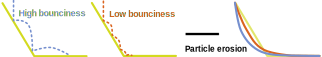
\includegraphics{bounciness.pdf}
\caption{The coefficient of restitution affects the amount of energy absorbed from the particle when hitting the ground. Here, rain is applied on an initial slope (yellow). Only two particles are displayed, with a high (blue) and low (red) coefficient of restitution. The resulting slope after erosion is displayed in blue and red (right). }
\label{fig:erosion_coefficient of restitution-diagram}

\end{figure}

\subsubsection{Velocity field}
\label{sec:erosion_velocity_field_refinement}
In our model, we allow the user to add a velocity field to the environment that influences particles motion. This velocity field can be the result of a complex fluid simulation, a uniform vector field, or an artistic motion field.
We modify Equation \eqref{eq:erosion_velocity-computation} such that the particle's speed will be influenced by the velocity field as follows:
\begin{align} \label{eq:erosion_velocity-computation-final}
\velocity = \int{ \extForce \, dt} + \settlingVelocity + \alpha \fluidVelocity + \velocity_0,
\end{align}
with $\fluidVelocity$ medium velocity field modulated by $\alpha \in [0,1]$. 

Our particle system can model intricate scenarios, like the erosion caused by water currents on the seabed or aeolian erosion. The velocity field remains static during the erosion, which may cause inconsistencies in the fluid velocity field. However, minor changes can be overlooked to maintain a balance between realism and computational efficiency \cite{Tychonievich2010}. We offer several velocity improvement methods: 
\begin{Itemize}
    \Item {Fluid simulation refinement:} Many erosion systems incorporate fluid simulation, requiring regular updates for erosion and velocity \cite{Kristof2009, Wojtan2007}. Our method can use fluid simulations with multi-resolution refinement, with the possibility to focus the velocity field adjustments near the updated boundaries of the surface \cite{Roose2011}. 
    
    \Item {Particle velocities in fluid simulation:} With a Lagrangian fluid simulation relying on particle systems \cite{Koschier2022}, our particle velocities can be incorporated in its computation. This approach is only a provisional solution due to potential parameter mismatches with main fluid simulation. 

    \Item {Velocity field diffusion:} Given the minor changes to the surface level at each erosion iteration, which reflect the gradual alterations in terrain surface, we can estimate that the velocity at a fixed point transitioning between the inside and outside of the terrain closely mirrors the velocities observed in its surrounding area. In this context, we can simply interpolate the velocity field at any transitioning point. This simple method, as used in \cref{fig:erosion_underwater_result}, allows us to find a balance between achieving realistic flow simulations and maintaining computational efficiency.
\end{Itemize}
% Our contribution part
% ------------------------------------------------------------
\section{Our erosion method}
\label{sec:erosion_application_on_representations}
\begin{figure}[ht]
    \centering
    
\includegraphics{figure_pipeline.pdf}
    \caption{Our overall pipeline: our erosion process compute matter displacement of a terrain using an arbitrary representation as long as intersections between particles and the ground can be detected. An optional velocity field, provided by the user, guides the particles trajectories. We propose surface alteration methods to apply the erosion to the terrain in a coherent way between possible representations. }
    \label{fig:erosion_figure_pipeline}
\end{figure}
In this section, we describe how to apply detachment and deposition to different terrain representations with our method (\cref{fig:erosion_figure_pipeline}). We cover the most commonly used representations namely height fields, layered terrains, voxel grid and implicit surfaces, note that our work could be extended to additional representations. Two conditions need to be satisfied for a representation to be eligible for our erosion method: being able to evaluate the intersection of a particle with the ground and compute the normal of the terrain at this point. To the best of our knowledge, all representation do. \\
We use Verlet integration for the particle's physics  \cite{Verlet1967}, with low error rate and stability even for high $dt$, reducing computation time for negligible imprecision \cite{Baraff1998, Swope1982}.

For all the representations, the amount of material absorbed by the particle, i.e. the erosion value $\erosionAmount$ from \eqref{eq:erosion_erosionAmount}, is taken around the particle at a radius $\particleSize$, meaning that the modification of the terrain by a particle at position $c$ will only occur for the positions $\p$ satisfying $||\p - c|| < \particleSize$. At the same time, the amount $\depositAmount$ from \eqref{eq:erosion_deltaDepositon} is deposited, resulting in a change $\totalErosion = \depositAmount - \erosionAmount$\\ 
In our simulation, while the dynamics are informed by physical principles, the particle size is conceptualized within a dimensionless framework. This provides the flexibility to adapt our results to various real-world scales, ensuring the applicability of our model across diverse scenarios.
Note that, for a 2.5D terrain, we can consider that half of the sphere surrounding the particle is affected which has a volume of $V_{2.5D} = \frac{2 \pi \particleSize^3}{3}$ while a 3D terrain is affected by the full sphere $V_{3D} = \frac{4 \pi \particleSize^3}{3}$ (as illustrated  \cref{fig:erosion_erosion_heightfield}). In the following sections, we will describe the strategies used to modify the amount of matter for different representations. 
\begin{figure}
\centering
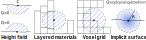
\includegraphics{a_erosion_deposition.pdf}
\caption{Illustration of the material detachment in the (half-)sphere at contact point $C$ (cross) on different representations. (height field) When $\totalErosion < 0$ material detachment happen in the bottom scaled half sphere of the particle's contact with the ground, while the deposition is applied on the upper half sphere of volume when $\totalErosion > 0$. Unlike the height field, for 3D terrains detachment and deposit are applied in the full sphere around the contact point.}
\label{fig:erosion_erosion_heightfield}

\end{figure}
\subsection{Application on height fields}
\label{sec:erosion_application_on_heightmaps}
On a height field defined by $h(\p) = z$, the intersection point with the surface is verified at $\p_z = h(\p)$, and the normal can be computed at the intersection point. 

For this representation, the half sphere is scaled in the $z$ direction to fit $\alpha \volume = \totalErosion$ using $\alpha = \frac{\totalErosion}{\volume}$. We then can decrease the height $h'(\p)$ at all points $\p$ by the height of the scaled half sphere at position $\p$. Given the height of the scaled half sphere of center $c$ and the distance of the particle to the center $d = ||\p - c||$ by $h_\text{half sphere}(\p) = \alpha \sqrt{\particleSize^2 - d^2}$ for all $\p$ such that $d \leq \particleSize$ the radius around a particle.

This change of height can be sampled at all points of the 2D grid by reducing the height by 
\begin{align} 
\label{eq:erosion_erosionHeightfield}
\Delta h(\p) &= \frac{\sqrt{\particleSize^2 - d^2}}{\alpha} = \frac{\totalErosion}{\frac{2}{3} \pi \particleSize^3} \sqrt{\particleSize^2 - d^2}
\end{align}
The height at each point after an erosion is then computed as $\Tilde{h}(\p) = h(\p) + \Delta h(\p)$.

\subsection{Application on layered terrains}
\label{sec:erosion_application_on_layers}
Layered terrains are defined as $\mu: \R^3 \to \N$ assigning a discrete material index $\mu$ for any point in space \cite{Benes2001, Peytavie2009}. In the original work, outer borders stack elements of the terrain are transformed into density-voxels to enable global erosion through height changes. We enable the erosion/deposition process directly on the layers hence removing the need for representation changes. \\ 
When intersecting the terrain, the amount eroded for each material stack should be the integration of the volume of the intersection between the sphere surrounding the particle and the cubicle represented by the stack. Since there is no easy solution \cite{Jones2017}, we approximate the volume of the stack we need to alter using the previously defined height field equation \eqref{eq:erosion_erosionHeightfield}. 
At a distance $d$ from the particle, the height is defined as:
\begin{align} \label{eq:erosion_erosionLayers}
H(d) = \frac{|\totalErosion|}{\frac{2}{3} \pi \particleSize^3} \sqrt{\particleSize^2 - d^2}.
\end{align}
If $\totalErosion > 0$ (more deposition is applied that detachment) then we transform the materials in the stack contained in the sphere to become ground material. For $\totalErosion < 0$ the materials are transformed in background material.

\subsection{Application on implicit terrains}
\label{sec:erosion_application_on_implicit}
Implicit terrain are defined using a function $f(\p)$ and its variation resulting from the erosion process using $\Delta f(\p)$.
We propose a strategy to compute $\Delta f(\p)$ at any point of the sphere surrounding the erosion point based on metaball primitives. At each contact point a metaball is added to create a hole or a bump in the terrain. A metaball is defined as: 
\begin{align}\label{eq:erosion_erosionMetaball}
\Delta f(\p) = \frac{3 \totalErosion}{\pi} \frac{(1 - d)}{\particleSize}
\end{align}
with $d$ the distance of the point $\p$ to the sphere center. For all point $\p$ for which $d \geq \particleSize$, $\Delta f(\p) = 0$ (see \cref{sec:erosion_appendix_metaball}).

As they are the most commonly used representations, we propose a formulation to erode implicit terrains defined by Signed Distance Functions (SDF) and by gradient or vector fields.

\subsubsection{Signed Distance Functions}
\label{sec:erosion_application_on_sdf}
Considering SDF, the terrain is defined as the 0-set of the signed distance function $f: \R^3 \to \R$, hence, for $f(\p) = 0$, the inside as $f(\p) < 0$ and outer-part (i.e. air or water) as $f(\p) > 0$. \\ 
The particle erosion applies at impact points at discrete positions, so we propose to add or subtract metaballs defined using equation~\eqref{eq:erosion_erosionMetaball} to respectively deposit or erode material using a composition tree:\\ $metaball(\p) = -\Delta f(\p)$.\\
Now the eroded terrain function $\Tilde{f}(\p)$ will be evaluated at each point $\p$ from the initial terrain value $f(\p)$, the erosion function $metaball(\p)$ and the composition function $g(f_1, f_2)$:
\begin{align} \label{eq:erosion_finalMetaball}
\Tilde{f}(\p) = g(f(\p), metaball(\p)).  \nonumber
\end{align}
As a metaball is added for each particle bounce on the terrain space partitioning optimization algorithms such as k-d trees, BSP trees or BVH can easily be used to improve performances.

\subsubsection{Other implicit terrains}
\label{sec:erosion_application_on_other_implicit}
are present in the literature, notably a 2.5D representation based on the surface gradient \cite{Guerin2022} and a 3D representation based on curves \cite{Becher2017} for which the trajectory of each particle projected to the closest surface could be used to define the alteration of the terrain.\\
In the case of gradient-based representation, we propose to use the partial derivative from the equation of the 2D scalar fields \eqref{eq:erosion_erosionHeightfield} that gives:
\begin{align} %\label{eq:erosion_erosion_gradients}
\nabla h' = - \frac{\totalErosion}{\frac{2}{3}\particleSize^3} \frac{1}{\sqrt{\particleSize^2 - d^2} } \vec{CP}
\end{align}
with $\vec{CP}$ the vector from the position $\p$ to evaluate to the center of the erosion point $c$.
Now the new gradient field can be computed as: 
$$
\nabla \Tilde{h}(\p) = \nabla h(\p) + \nabla h'(\p).
$$
\begin{figure*}
\centering
\includegraphics{new_continuous_erosion2.png}
\caption{Our erosion method is applied iteratively on a completely synthetic island, the terrain is altered to obtain a plausible shape by forming rills. The use of particles with hydraulic densities dropped from the sky results in a strong erosion on the sides of the mountains, and the particles that slide to the sea are mainly drifting offshore resulting in the formation of small beaches and a weaker erosion on the bottom of the water body. Repeating the process causes the island height to decrease progressively up to the point where only the submerged part of the terrain is sheltered from erosion.}
\label{fig:erosion_continuous-erosion}

\end{figure*}

\subsection{Application on voxel grids}
\label{sec:erosion_application_on_voxels}
% \subsubsection{Density-voxels}
We consider two of the voxel grids representations: density-voxel grids and binary voxel grids for which we present our material alternation strategy.

\subsubsection{Density voxels}
\label{sec:erosion_application_on_density_voxels}
We consider "density-voxel" grids defined on $f: \Z^3 \to [-1, 1]$ for which a voxel is be full for $f(\p) = 1$, partially full for $-1 < f(\p) < 1$ or empty for $f(\p) \leq -1$. 
This definition allows us to erode them smoothly. 
Since this kind of grid is a discretizaion of a scalar function, We could directly use \eqref{eq:erosion_erosionMetaball}, as described previously, but we take advantage of the discrete nature of the representation to avoid expensive computation. \\
We apply the erosion from a particle at position $c$ on all points $\p$ in the volume proportionally to the distance from the center of the sphere $d = ||\p - c||$ to find an approximation to the real erosion value per voxel $\totalErosion_{approx} = \totalErosion \frac{1 - d}{\particleSize}$.
Using their discrete nature, we rectify this value to sum up the total erosion value to $\totalErosion$ by dividing each value by the sum of the distances. We now consider eroding the "empty" voxels since their density can drop until $-1$. We then have for all surrounding voxels: 
\begin{align} \label{eq:erosion_erosionVoxels}
\Delta f(\p) = \totalErosion \frac{ (1 - \frac{d}{\particleSize} )}{ \sum {(1 - \frac{d}{\particleSize})}}.
\end{align}
Resulting voxel value is computed as $\Tilde{f}(\p) = f(\p) + \Delta f(\p)$.
In our implementation, when $f(\p) > 1$, we simply transport the density excess to the above voxel, giving it a very close analogy to height fields as long as $|\Delta f| < 1$. 

\subsubsection{Binary voxels}
\label{sec:erosion_application_on_binary_voxels}
The terrain can be represented using an occupancy function as $f: \Z^3 \to \{0, 1\}$ where a voxel $f = 1$ defines the ground and $f = 0$ the background. \\ 
We propose to apply particle erosion by assigning voxels a number of hits, and transform them as air or as ground when this number reaches a critical value $C$ that is proportional to the particle's strength parameter $\erosionStrength$ \cite{Jones2010}. \\ 
On a hit, all voxels in a radius $\particleSize$ receive a hit number: 
\begin{align} \label{eq:erosion_erosionDiscreteVoxels}
\Delta hits = \lfloor \alpha \Delta f \rfloor
\end{align}
with $\Delta f$ the erosion per voxel computed using \eqref{eq:erosion_erosionVoxels} and $\alpha$ a coefficient high enough to obtain values above 1. \\ 
All voxels with $\# hits > C$ are transformed to background and voxels with $\# hits < -C$ are transformed to ground.\\
Note that, a binary voxel grid can also be transformed into a density-voxel grid to be eroded smoothly.

Our formulation for height fields \eqref{eq:erosion_erosionHeightfield}, can be used to erode 2D scalar field-based representations. Similarly, 
our proposition for SDF \eqref{eq:erosion_erosionMetaball} enables erosion for continuous 3D scalar fields and voxels \eqref{eq:erosion_erosionVoxels} for discrete 3D scalar fields respectively.
% -----------------------------------------------------------
\section{Results}
\label{sec:erosion_erosion_examples}
% \begin{wrapfigure}{r}{3,5cm}
% \centering
% \includegraphics{multi_representations.pdf}
% \label{fig:erosion_comparison-representations}
% \end{wrapfigure}
Our erosion process enables the simulation of a wide range of erosion effects on the major terrain representations alike. In this section, we present applications that demonstrate the versatility of our method by changing the particle's effect size, quantity, density, maximum capacity, deposition factor and the velocity fields. The results of each process are presented in \cref{tab:erosion_result_figures}, parameters used are available at \cref{tab:erosion_result_parameters}. 
It is important to note that all erosion examples presented in this section are available for any 3D terrain representation. However, we cannot create volumetric structure, such as overhangs, using 2.5D representations (height fields).

Environment density $\fluidDensity$ is set to \SI{1}{\kilogram\per\cubic\meter} above water level (terrain blue part) and to \SI{1000}{\kilogram\per\cubic\meter} below it.
Velocity field's refinement is done by using the presented diffusion strategy.

\afterpage{
\begin{landscape}
\begin{table}%[htbp]
    % \centering
        \begin{tabular}{|lHlllllllllllll|}
            \hline
            \thead{Name} & \thead{Results} & \thead{Rep.} & \thead{Dimensions} & \thead{Res} & \thead{$\#P$} & \thead{$\#N$} & \thead{$\particleSize$} & \thead{$COR$} & \thead{$\particleDensity$} & \thead{$\capacityFactor$} & \thead{$\erosionRate$} & \thead{$\depositionRate$} & \thead{Vel field} & \thead{$t$} \\
            \hline
            \exampleHydraulic \\
            \exampleCoastal \\
            \exampleMeanders \\
            \exampleRiverTwo \\
            \exampleLandslide \\
            \exampleVolcano \\
            \exampleKarstBinary \\
            \examplePipes \\
            \exampleWindErosion \\
            \exampleWaterCurrents \\
            \hline
        \end{tabular}
        \caption{Parameters used for the generation of the terrains presented in \cref{tab:erosion_result_figures}, with "Rep" the representation  (\heightmap: Heightmap, \densityVox: Density-voxels, \binaryVox: Binary voxels, \implicit: Implicit) "Res" the resolution in meter per voxel or cell, $\#P$ the number of particles per iteration, $\#N$ the number of iterations, $\particleSize$ the particles radius (in voxel or cell unit), $COR$ the coefficient of restitution, $\particleDensity$ the particle density in \SI{}{\kilogram\per\cubic\meter}, $\capacityFactor$, $\erosionRate$ and $\depositionRate$ respectively the capacity, erosion and deposition factors, "Vel field" the type of velocity field used and $t$ the computation time of the simulation in seconds on CPU. \\ $^{(1)}$ The velocity field is a vector field defined as $\fluidVelocity(\p) = [0 ~ sin(\p_x) ~ 0]^T$.}
        \label{tab:erosion_result_parameters}
\end{table}
\end{landscape}
}

\subsection{Rain}
Hydraulic erosion from rain is the most common process used in terrain generation. In this case, particles are seen as water droplets falling from the sky and rolling downhill due to the gravitational force of Earth. No velocity field is required from fluid simulation. These parameters result in a detailed geometry of the rills on the side of mountains that quickly emerge and deposit many sediments in the valley.  
We demonstrate the result of rain erosion in \referenceExemple{Rain} with a computation time of 4 seconds.  \\
Using this erosion parameters in combination with water bodies results in different outcomes (\cref{fig:erosion_continuous-erosion}). The terrain above water is directly affected by the erosion process while particles colliding with the underwater part of the terrain are slowed down and filled with sediments, leading to mainly apply deposition. The result is a typical hydraulic erosion on mountains and the formation of slopes and beaches near water level.

\subsection{Coastal erosion}
Waves repeated motion  creates coastal erosion, that can be seen as cliffs with holes at the water level. \\
We apply a uniform velocity field in the water pointing towards the coast to simulate waves and emit particles from the water area with a large size, a density between air and water densities, a high capacity factor and a low deposition factor $\depositionRate$. Using these parameters, the erosion process is focused at the interface of air and water, and apply a coarse detachment while depositing a very small quantity of sediments, simulating the corrosive effect of water on limestone. \\ 
This effect can only be simulated on 3D terrain representations, but will create cliffs on a 2D representation. 
\referenceExemple{Coastal} presents the result of coastal erosion on a density-voxel grid that creates overhangs around sea level using a small amount of particles. Note that, the same effect using an alternate implicit representation based on SDF is displayed in \cref{fig:erosion_screen-paris2019-1}.
A shaded version of this effect is presented in \cref{fig:erosion_closerImage}.

\subsection{Rivers}
Given a source point, we generate particles that run downhill, simulating the formation of a river. More complex erosion simulation using fluid simulations like SPH \cite{Kristof2009} would create realistic results at the cost of high processing time. Our method offers the flexibility to be applied either with a velocity field (simple, used given or resulting from a fluid simulation) or without allowing for simplicity and efficiency.\\
When provided with a hand-made or procedural velocity field, our particle system can reproduce simple river meanders (\referenceExemple{Meanders}). \\ 
\referenceExemple{River} presents a river that has been modeled by emitting water particles with different sizes that ranges from \SI{1.5}{\meter} to \SI{5}{\meter}, a high coefficient of restitution and a low capacity factor. Random sizes are used to simulate a river for which the flow rate had fluctuated over formation time, while the low capacity ensure that the banks of the river stays smooth. A high coefficient of restitution is a strategy that let the particles flow with low friction, approaching a water behaviour. Our particles are affected only by gravity, without fluid simulation.

\subsection{Landslide}
are mainly caused by large amount of water saturating the ground and flowing downhill, transporting matter in its path. \\
By using water particles with a medium size, a low coefficient of restitution and a low capacity factor but a high deposition factor $\depositionRate$, they transport sediments on short distances as the velocity quickly drops to 0, and ground material is completely spread along its path since it is easier to deposit the same amount of sediment than the eroded amount at each collision point. Reducing the density of the particle simulates a rise of viscosity in the settling velocity formula, increasing again the quantity of matter to deposit at contact with the ground. By this means, we can simulate landslides as illustrated on \referenceExemple{Landslide}. A smoother surface is resulting, compared to the rain erosion as the rills are filled with sediments as soon as they begin to form.
%
By setting the initial capacity of the particle equal to 10\% of its max capacity, the mass of the terrain increases, simulating a volcano eruption as illustrated on \referenceExemple{Volcano}.

\subsection{Karsts} networks are created over hundreds of years from the corrosion of water on the limestone in the ground. A limited number of methods have been proposed for the procedural generation of karsts \cite{Paris2021}.\\ 
By reducing the deposition factor $\depositionRate$, the particles simulate corrosion (without mass conservation). We can use the same particle parameters than the coastal erosion (big size, a density between air and water densities, a high capacity factor and a low $\depositionRate$) and optionally provide a 3D shear stress map. The karst will automatically follow the softest materials, which is geologically coherent as given in example in \referenceExemple{Karst}, where we can observe a "pillar" that is formed in the center, and thus the karst forms two corridors that finally merge partially. 
%
Underground results are only available for representations allowing 3D structures. Another underground terrain simulation is shown in \referenceExemple{Tunnel} in which a water runoff is eroding a tunnel without the use of a fluid simulation. Here, when particles bounce often on the terrain surface, the coefficient of restitution may be seen as a viscosity parameter.

\subsection{Wind}
erosion is a significant process in desertscapes shaping since there are no obstacles on the airflow path. Air particles can reach high velocities, transporting sand over long distances forming either dunes or are blasted into rocks, eroding into goblins. \\ 
By setting the density of our particles close to \SI{1}{\kilogram\per\cubic\meter}, two erosion simulations can be applied at once. Air particles follow closely the flowfield given by the user in air. This flowfield can be given from a complex simulation, a user-defined wind rose \cite{Paris2020} or a random flowfield with a general direction. \\ 
The generation of the different sand structures depends on the velocity field provided, and a simple field will easily generate linear dunes. On contact with a rock block, the simulation will automatically erode block borders, creating shapes looking like gobelins. \\
\referenceExemple{Wind} gives an example of wind erosion on a flat surface with rock columns being eroded. Given a strong 2D velocity field computed by the high wind simulation proposed in \cite{Paris2020} is used on light particles, the simulation is fast thanks to the low number of collisions each particle has with the ground. 

\subsection{Underwater currents}
Procedural generation of underwater 3D terrains has received little attention. The difference between the underwater and the surface rely on the buoyancy force that is much stronger, meaning that the water flow has a much more impacting effect on erosion than wind. Taking into account the density of the environment and the velocity field of water in our formulas are the keys to be able to apply any erosion in this environment. 
Our method works in a water environment by giving at least water density to particles. Given a velocity field describing underwater currents from a complex simulation or from a sketch, the particle system erodes the terrain. \\ 
In the example presented in \referenceExemple{Underwater}, the velocity field is given by a simple 3D fluid simulation \cite{Stam1999} applied on the terrain.

A complex water flow simulation is computed using SIMPLE \cite{Caretto1973} fluid simulation with OpenFOAM. The resulting erosion can then follow complex water movement and erode the terrain at the most affected parts of the 3D terrain as the trajectories of the particles (green) is highly affected by the fluid velocity (blue). The density of the particles and the environment being close, the buoyancy cancels most of the gravity force, leaving the velocity of the particles computed by the fluid velocity $\fluidVelocity$ and settling velocity $\settlingVelocity$ from \eqref{eq:erosion_velocity-computation-final} (\cref{fig:erosion_underwater_result}).
\begin{figure}[ht]
    % \centering
    \includegraphics{flowfield.pdf}
    \caption{A complex water flow simulation is computed using OpenFOAM. Particle trajectories (green) are highly affected by the fluid velocity (blue). Most the terrain exposed surfaces is eroded (bottom). }
    \label{fig:erosion_underwater_result}
\end{figure}


\subsection{Multiple phenomena} 
A terrain eroded with multiple erosion phenomena applied on a 500x500x50 density-voxel grid is illustrated in \cref{fig:erosion_multiErosions}. Here, water-density particles are applying rain on the terrain while the coasts of the river are being eroded thanks to a velocity field defined at the water level. The velocity field defined in the air mainly affects particles with air-density, such that wind erosion can be applied at the same time. The computation of these effects took 7 seconds on CPU.

\begin{figure}[ht]
    % \centering
    \includegraphics[width=0.49\linewidth]{MultiEffects_base.png}
    \includegraphics[width=0.49\linewidth]{MultiEffects.png}
    \caption{Multiple erosion types can be combined. On an initial synthetic 500x500x50 density voxel grid, the a wind erosion is applied on the surface of the terrain while hydraulic erosion shapes the rills and the base of the mountains. A water current digs its borders and spreads sediments at the bottom. }
    \label{fig:erosion_multiErosions}
\end{figure}

\section{Comparisons}
In the following section, we compare our method with existing ones to show that while we are versatile on the terrain representation, we are also able to reproduce various effects without applying specific algorithms. The other works are displayed in blue to distinguish them from ours.

\subsection{Coastal erosion on implicit terrain representation}
\citep{Paris2019} present an erosion simulation method applied to implicit terrains able to create coastal erosion, karsts and caves by adding negative sphere primitive in the terrain's construction tree. The positions of the spheres are determined using a Poisson disk sampling at the weakest terrain area defined by the Geology tree of their model. They are simulating the corrosion effect of water on the rocks. Our work is also able to approximate this phenomena by defining the position of these sphere primitives at the position where the water particles hit the surface. While the computation time of the positions of the sphere is higher due to the fact that we are evaluating the position of our particles at every time step in the implicit model (which could be improved by the triangulation of the implicit surface, or better, a dynamic triangulation), the distribution of our erosion primitives is based on a physical model instead of a mathematical model, meaning that we can integrate more easily the direction and strength of the waves for example. The management of their sphere primitives can be replicated with our method by considering that a particle exists until a collision occurs, at which point it disappears. Their method is not conserving the mass of the terrain, which is acceptable for the corrosion simulation, but limits its validity for other erosion simulations. In our method, the particle can be tracked until it settles, ensuring mass conservation (\cref{fig:erosion_screen-paris2019-1});

\begin{figure}
\centering
\includegraphics{costal.pdf}
\caption{The algorithm proposed by \cite{Paris2019} allows for the simulation of coastal erosion (left) that we can reproduce almost identically by allowing our particles to collide only once with the ground and applying only erosion (center). If we apply our erosion with the full tracking of our particles and using deposition, we can achieve more diverse results (right).}
\label{fig:erosion_screen-paris2019-1}
\end{figure}

\subsection{Wind erosion on voxel grid representation}
\citep{Jones2010} propose a weathering erosion on voxel grids by approximating and eroding continuously the most exposed voxels. When a solid voxel is decimated, it is considered deposit and is displaced down the slope until a minimal talus angle in the terrain is reached and if the deposition is eroded again, it disappears. Our work is able to reproduce their algorithm by sending our particles from a close distance to the terrain surface. By doing so, we reproduce the erosion process as much as the deposition process since the air particles, filled with sediments, is falling automatically towards the local minimum of the erosion point. Just like in their work, we can easily define the resistance value of the materials to add diversity in the results. By adding the possibility of a wind field, even a very simple uniform vector field, to the simulation, we naturally add the wind shadowing effect that protects a gobelin surrounded by bigger gobelins, and also allows the deposit slope to fit more closely to the wind direction (\cref{fig:erosion_screen-jones2010}).

\begin{figure}[ht]
    \centering
    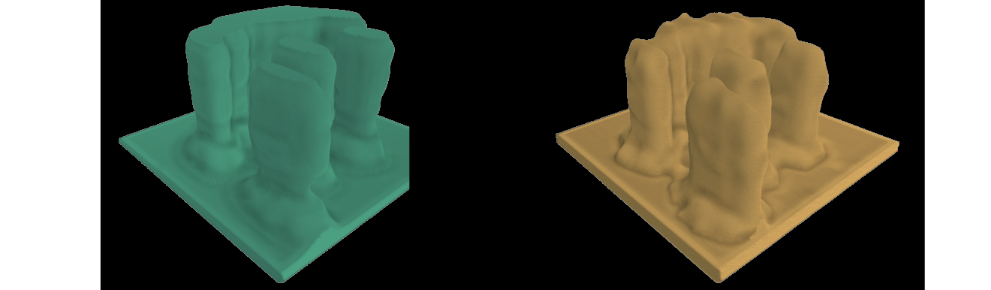
\includegraphics[width = \linewidth]{gobelins2.png}
    \caption{The algorithm proposed by \cite{Jones2010} allows for an efficient simulation of the spheroidal erosion, making the creation of gobelins on voxel grids in a plausible way (left). Our algorithm naturally erodes the most exposed areas of the terrain when particles are affected by the wind (right).}
    \label{fig:erosion_screen-jones2010}
\end{figure}

\subsection{Hydraulic erosion on height field representation}
\citep{Mei2007} integrate and adapt to the GPU the pipe model proposed in \cite{OBrien1995} for the fluid simulation. This simulation is simple but efficient enough to approximate the Shallow-Water equations in real time and use the speed of columns of water to compute the erosion and deposition rate on the 2D grid of the terrain at each time step. Using columns of water even allows the flow to overpass small bumps on the terrain over time. Our method initially rely on a stable fluid flow that is consistent during the whole life time of a particle, but by refining the simulation at each time step instead of at the end of the particles lifetime, our erosion model is able to reproduce this effect, allowing the terrain to have a single batch of fluid going through it. Our method can be seen as a generalization of Mei at al. that can then be used on more than discrete 2D grids (\cref{fig:erosion_screen-mei2007-1}). 

\begin{figure}[ht]
    \centering
    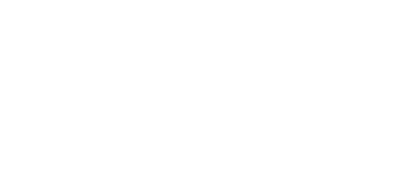
\includegraphics[width= 1\linewidth]{hydro.pdf}
    \caption{While our resulting geometry on the hydraulic erosion (bottom) is less smoothed than the one proposed proposed by \cite{Mei2007} (top), our method allows the application on more terrain representations than the height fields only.}
    \label{fig:erosion_screen-mei2007-1}
\end{figure}

\subsection{Wind erosion on stacked materials representation}
\citep{Paris2020} simulate the effect of wind over sand fields defined on stacked materials, creating dune structures, even taking into account obstacles like \cite{Roa2004} and different material layers like vegetation \cite{Cordonnier2017a} that are not affected by abrasion\cite{Paris2020}. A wind field simulation is required to produce results, and while \cite{Roa2004} and \cite{Onoue2000} consider a uniform vector field, this work consider a dynamic vector multi-scaled warped field from the terrain height. The sand grains then apply multiple moves: sand lift, bounces, reptation and avalanching. Once the sand is lifted by the wind, the trajectory of the grains can be seen as the displacement of particles, fitting completely with our model as illustrated \cref{fig:erosion_screen-paris2020}.
\begin{figure}[ht!]
\centering
\includegraphics{desert.pdf}
\caption{The algorithm from Paris 2020 allow the generation of desertscapes (top), which we can (at least partially) reproduce with our erosion simulation (bottom). The different effects are achieved by affecting the wind direction and strength. }
\label{fig:erosion_screen-paris2020}
\end{figure}

\section{Discussion}
This work is a generalization of erosion that is applicable to any terrain representation. In practice, while similar particle physics is used on different terrain representations, using similar parameters does not ensure resulting in the same eroded terrain. Surfaces and normals being approximated differently have rippling effect on particle trajectories. 
Note that, not all effects can be applied to all representations, forinstance, karsts generation on 2.5D data structures. 

\subsection{Realism}
Realism of the erosion simulation is highly correlated to the size and quantity of particles used and their distribution. Using too few or distributing them too sparsely will result in a terrain that is unrealistic since the alteration will have localized effects, breaking process homogeneity. \\ 
The resolution is also limited by the number and size of the particles, which can be problematic on implicit terrains that can theoretically have a infinite resolution.\\
Our method allows to perform erosion on implicit terrains. However, in its current form, our algorithm is time expensive on implicit representations since a large number of primitives are added in the composition tree. Using skeletons-defined primitives \cite{Hong2013, Rigaudiere2000}%, Schroeder1994}
 from particles trajectories and erosion/deposition values could be a solution to optimize the computation time.

\subsection{Usage of velocity fields}
In our erosion algorithm, we simplify particle physics to enhance computational efficiency and facilitate parameterization. We use the velocity field from fluid simulations to approximate particle velocities. Sediment mass is harnessed to compensate for this approximation, allowing compatibility with various fluid simulation algorithms. Velocity fields can be recomputed at a frequency meeting the applications needs, ranging from "classic erosion simulation" (recomputed at each time step) to "simple simulation" (never recomputed). We addressed provisional adjustments to mitigate discrepancies when terrain changes due to erosion are not reflected in a static velocity field in section “3.3 Transport”. However, it is important to note that these are expedient solutions and may not fully capture precise dynamics of an evolving terrain. 

\subsection{Performances}
To facilitate parallelization, we intentionally overlook particle interactions and sediment exchanges, albeit at the expense of achieving smoother results. Surface collisions are simplified to basic bounces with a damping parameter instead of relying on complex particles and ground properties (Young's modulus, friction, material, ...)\cite{Yan2020}, further easing the parameterization process. However, these simplifications, combined with the inherent discrete nature of particles, as opposed to the continuous nature of erosion, result in a correlation between realism and particle count. \\
The performance of our method is influenced by the time required for collision detection. Consequently, we mainly observe better performances with explicit terrain models than with implicit models. 

\subsubsection{Particle's atomicity}
While we can replicate various effects, the "fan" shape commonly observed in natural erosion patterns is not perfectly represented. This limitation arises because we do not account for the splitting of a particle, a process that significantly influences the multidirectional dislocation and trajectory of individual particles \cite{Ranz1960}. Additionally, we acknowledge an issue where particles may collide with the ceiling and the deposition is stuck. While a potential resolution involves splitting particles upon impact rather than simply depositing sediments, this introduces complexities to the parallelization layer of the method. Allowing particles to split introduces unpredictability in the total number of particles that will exist in the simulation. This unpredictability can complicate the use of multi-threading. Future works includes finding a data structure allowing this splitting efficiently, leading to more realistic erosion patterns.

\subsubsection{Simulation with multiple materials}
One aspect we haven't addressed is a layered terrain with multiple materials. In the native way our method is done, we do not consider the transport of different materials (all sediments are considered as sand), but by storing a list of the different materials and the quantity transported by each particle, the same simulation process could be done at the cost of some memory and performance overhead. \\
Another possible adaptation of the erosion strategy for material voxels is to extend the erosion computation from binary voxels by define transformation rules from one material to another when a voxel is eroded a number $\#hits < -C$ or $\#hits > C$. For example, the material "clay" may transform to "sand" when eroded or to "rock" when many depositions occurred. 
\section{Conclusion}
\label{sec:erosion_conclusion}
We introduced a flexible particle-based erosion system that is easy to use and simple to implement. We have presented how to adapt the process for various terrain representations and generate a variety of erosion phenomenon due to rain, wind, water bodies... by adjusting intuitive parameters hence generate automatically realistic 2.5D and 3D terrains. The use of external velocity fields provides a high flexibility i.e. using the simulations that best fits the user's needs (precision, control, implementation efficiency...). 
Our method can also be applied to underwater environments with identical physics simulation since our erosion method can be applied on 3D representations. 
Erosion algorithms are often limited to the use of height fields, but by finding more generalized methods, we can go toward a global use of 3D terrains, which can offer richer and more diverse landscapes.

\clearpage
\begin{figure*}
	\centering
    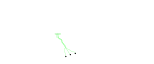
\includegraphics{results.pdf}
	\caption{Erosion processes results on various representations presented in section \cref{sec:erosion_erosion_examples}. Used parameters used are detailed in  \cref{tab:erosion_result_parameters}.}
	\label{tab:erosion_result_figures}
\end{figure*}
